\chapter{Evaluation}
\label{chap:evaluation}
In this chapter, we present the experimental results of the implemented detection methods. The evaluation is primarily based on tree performance metrics: precision, recall, and F1-score. By systematically comparing these metrics across the different methods, we are able to identify their respective strengths and limitations. This comparison further allows us to determine which approach achieves the best overall performance under the considered evaluation scenarios, as well as analyze the inherent trade-offs between detection accuracy and false positive or false negative rates. 

\section{Traditional \ac{ML} Detection Methods}
\subsection{F1-Scores}

\begin{figure}[!htbp]
	\centering
	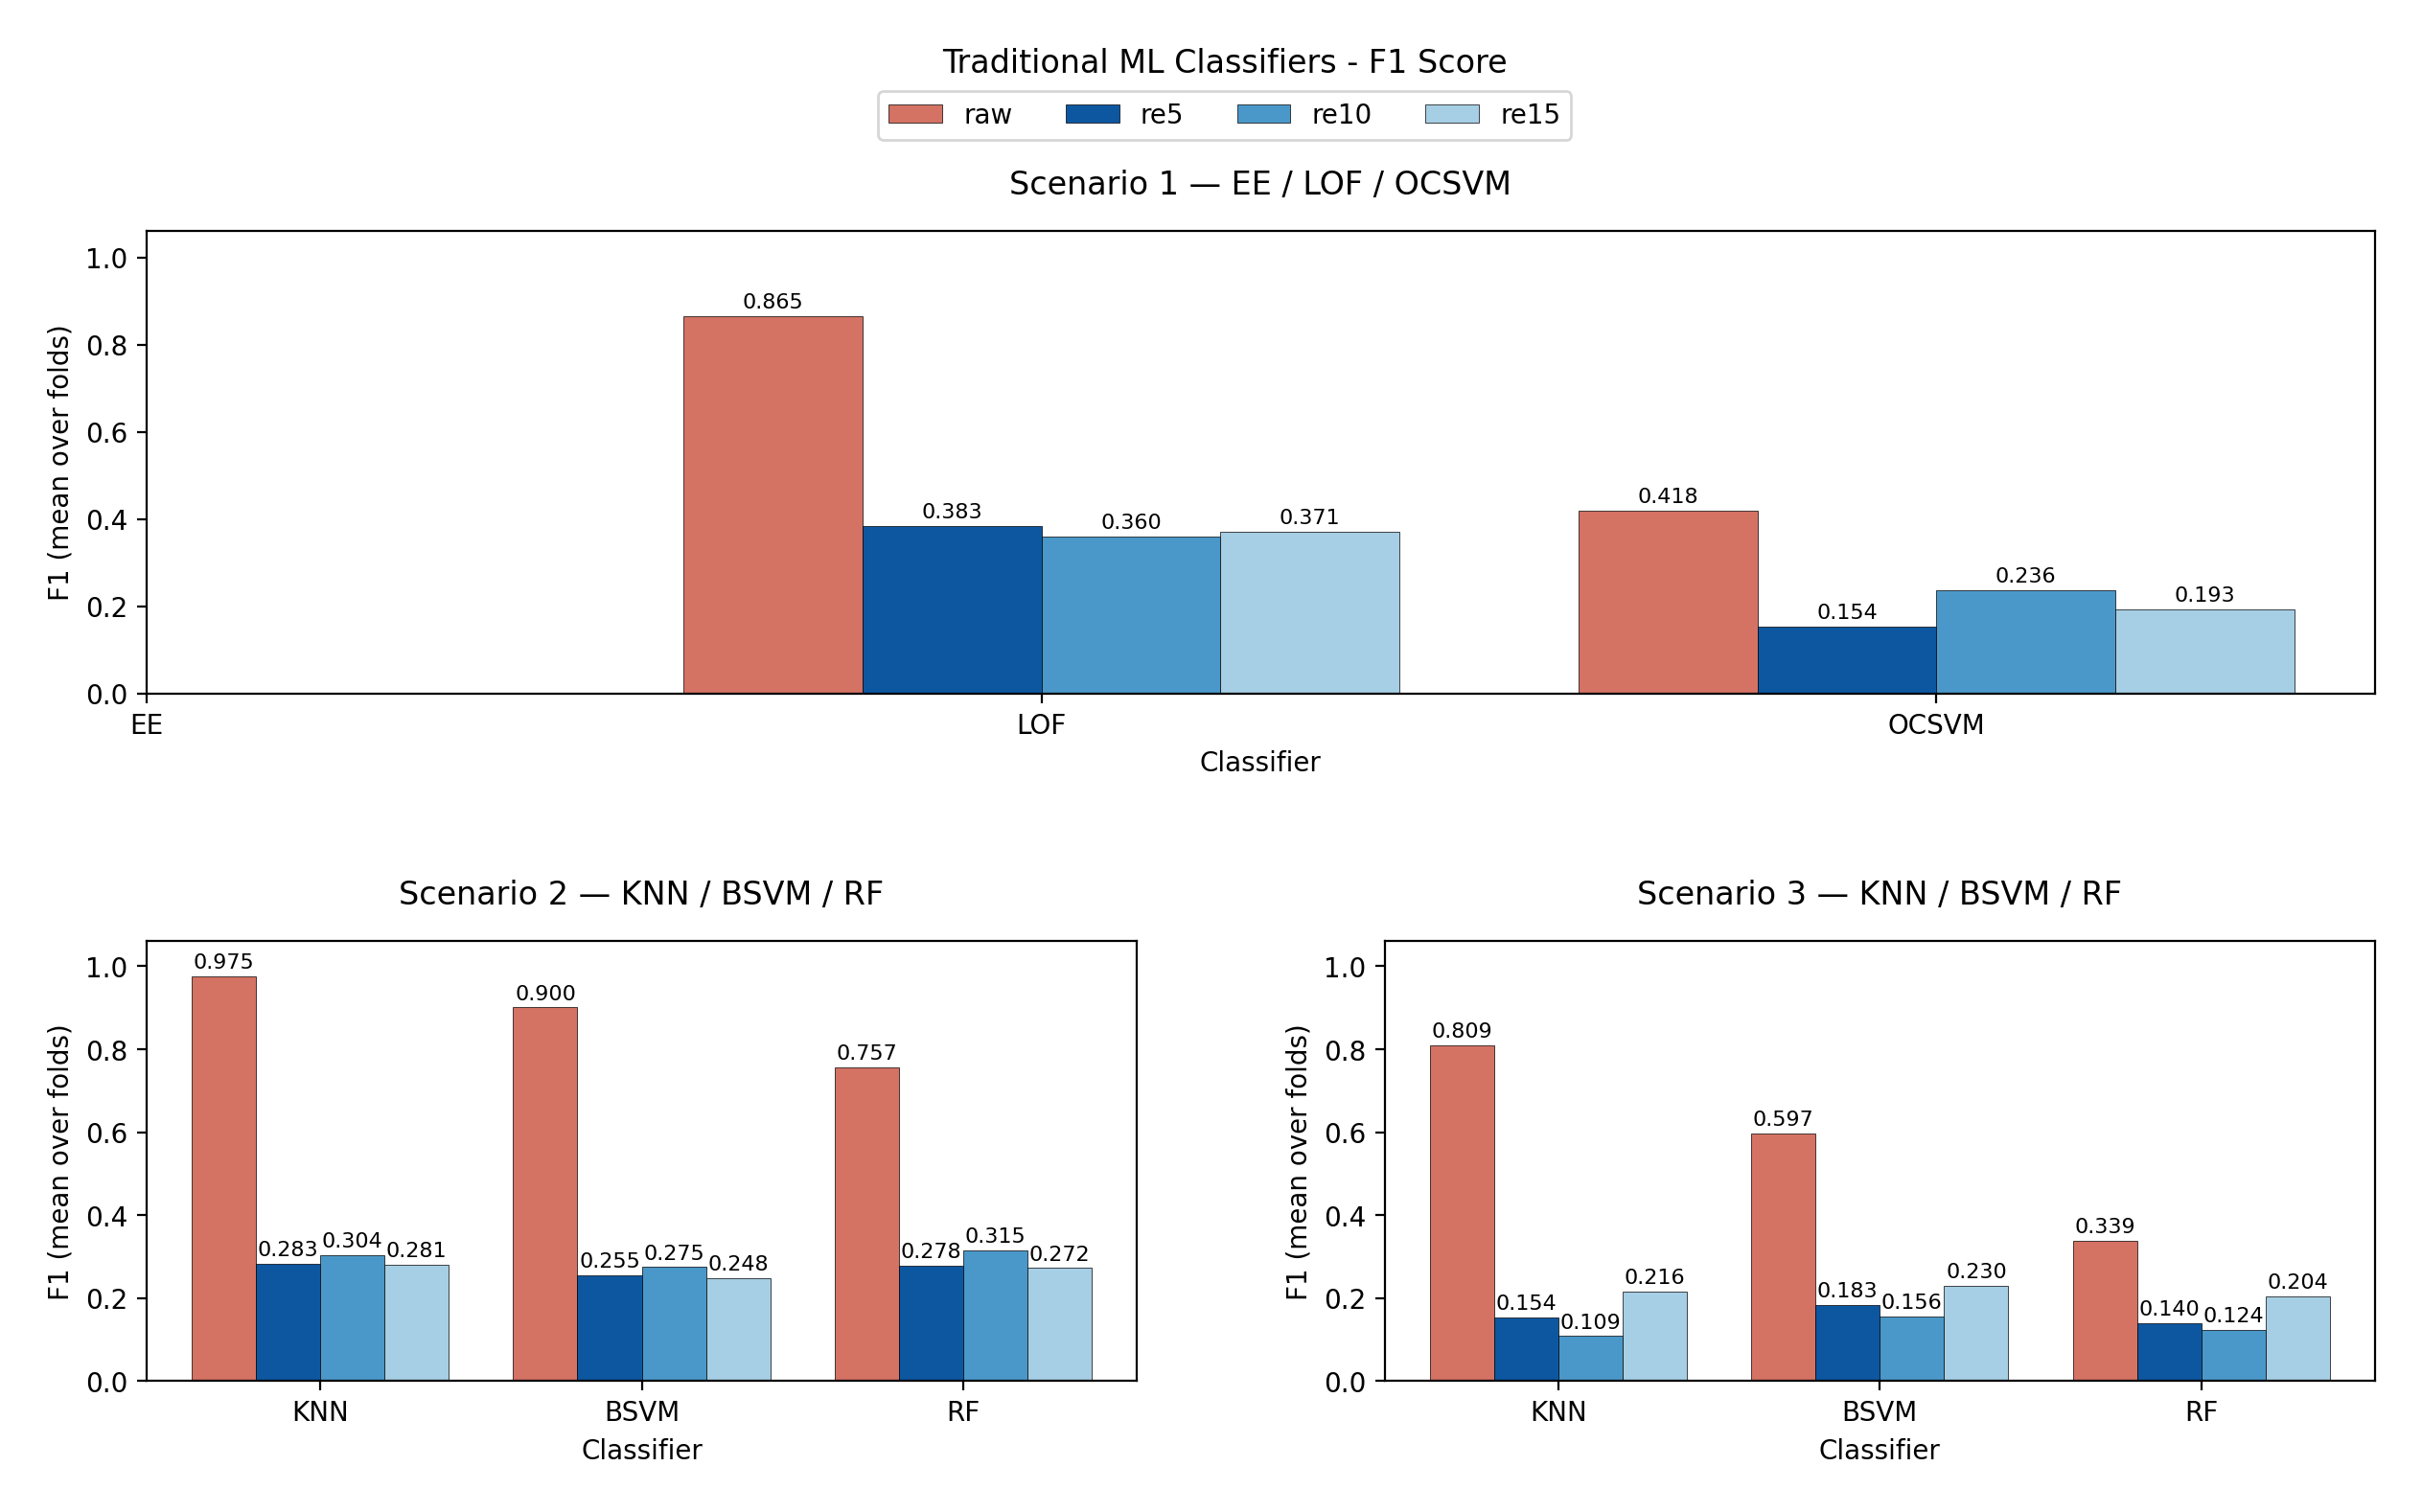
\includegraphics[width=\linewidth]{chapters/f1_custom_layout.png}
 \caption{Traditional ML Detection Methods F1-Score}
  \label{fig:tradML}
\end{figure}

figure \ref{fig:tradML} presents the mean F1-scores of the traditional machine learning
classifiers across the three evaluation scenarios. Scenario~1 evaluates
the one-class methods (Elliptic Envelope, \ac{LOF}, and One-Class \ac{SVM}),
whereas Scenarios~2 and~3 evaluate the supervised classifiers
(\ac{KNN}, Binary \ac{SVM}, and Random Forest). The different colors represent
the dataset representations (RAW, RE5, RE10, RE15).

For the RAW representation, \ac{LOF} achieves the strongest performance,
clearly outperforming Elliptic Envelope and One-Class \ac{SVM}.
In contrast, the latter two methods achieve only moderate performance.

When using the \ac{RE} representations, the performance
drops substantially for all one-class methods. In particular,
Elliptic Envelope fails to detect anomalies effectively, while
\ac{LOF} and One-Class \ac{SVM} achieve only low F1-scores. This indicates
that the reduced RE representations do not provide sufficient
discriminative information for one-class modeling.

In Scenario~2, all supervised classifiers achieve high F1-scores
when operating on the RAW representation. \ac{KNN} performs best,
followed closely by Binary \ac{SVM} and Random Forest.

However, when switching to \ac{RE}-based representations, performance
decreases significantly across all classifiers. Although minor
variations exist between RE5, RE10, and RE15, the results remain
consistently below the RAW baseline. This suggests that the full
packet structure contains important discriminative features that
are partially lost in the \ac{RE} representations.

Scenario~3 introduces previously unseen attack types during testing.
For the RAW representation, all supervised classifiers exhibit
a noticeable drop in performance compared to Scenario~2,
with \ac{KNN} remaining the strongest model.

Using the \ac{RE} representations further degrades performance.
In this setting, several classifiers approach near-random
behavior.


\subsection{Ensemble Classifier Results}

\begin{figure}[!htbp]
	\centering
	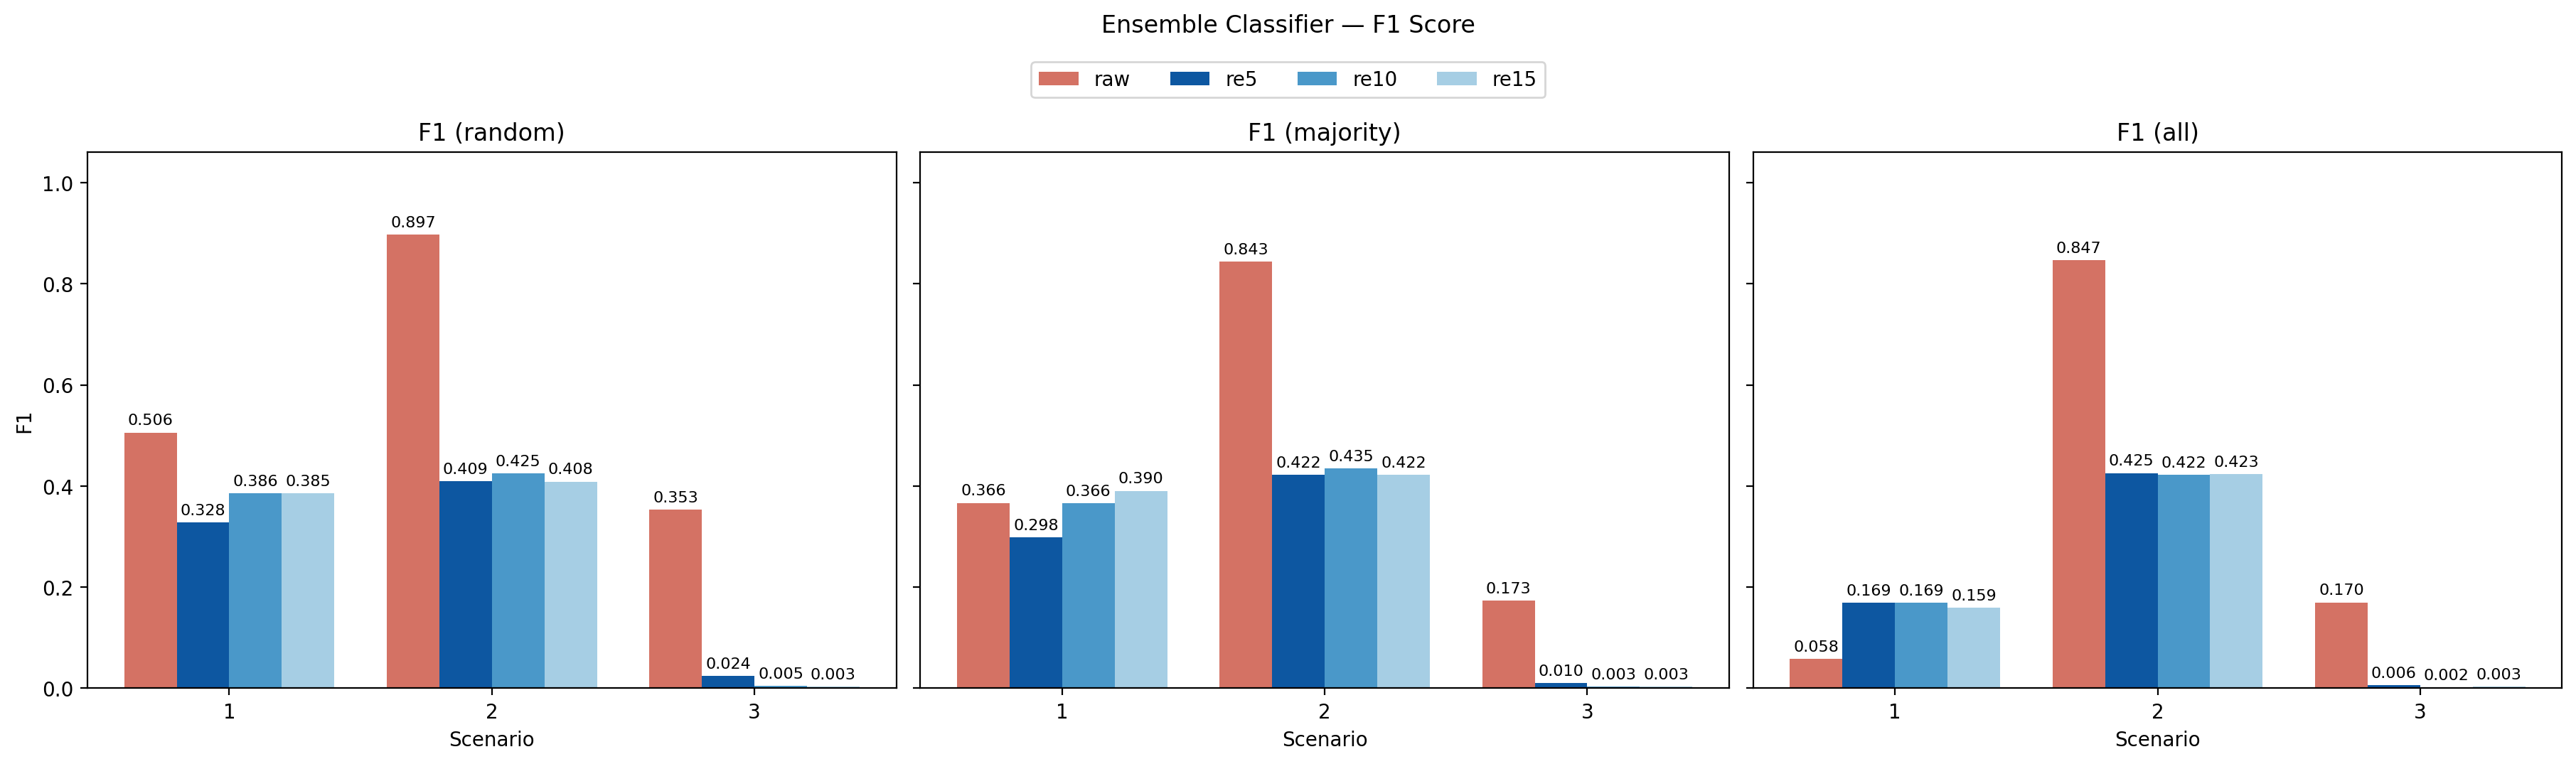
\includegraphics[width=\linewidth]{chapters/ec_all_representations_f1.png}
	\caption{Ensemble Classifier F1-Score}
 \label{fig:ec}
\end{figure}

figure \ref{fig:ec} shows the mean F1-scores of the ensemble classifier under
the three aggregation modes (random, majority, all) across all
dataset representations and evaluation scenarios.

Across all representations and aggregation modes, a consistent
difficulty ordering can be observed: Scenario~2 achieves the best
performance, Scenario~1 yields intermediate results, and Scenario~3
consistently performs worst. This pattern is stable across RAW and
all reverse-engineered representations, indicating that the scenario
characteristics have a stronger impact on performance than the
chosen ensemble strategy.

In particular, Scenario~3 leads to a substantial drop in F1-score
for all dataset types, reflecting the difficulty of generalizing
to highly constrained or unseen attack configurations.

For the RAW representation, the random and majority strategies
perform similarly and achieve strong results in Scenario~2.
In contrast, the \emph{all} strategy often leads to a noticeable
performance decrease, especially in Scenario~1. This behavior
suggests that at least one weak base classifier negatively
influences the ensemble when unanimity is required.

Overall, majority voting provides the most stable behavior
across scenarios, while the \emph{all} strategy appears overly
restrictive.

A clear performance gap is visible between RAW and all
reverse-engineered representations. The RAW dataset consistently
achieves substantially higher F1-scores across all scenarios and
ensemble modes.

The reverse-engineered representations (RE5, RE10, RE15) show
comparable behavior among each other, with RE15 generally yielding
the strongest results within this group. Nevertheless, their
performance remains significantly below that of the RAW data.


\clearpage
\subsection{Feature Importance}
To better understand which components of the 32-dimensional latent
feature vector drive the classification decisions, we analyze feature
importance for each traditional ML model. Each panel in the following
figures corresponds to one classifier and displays the importance
scores for all 32 features ($f_0$–$f_{31}$).

Since importance definitions differ between models and
are normalized independently (see \ref{subsubsec:feature_importance}), values should primarily be interpreted
within each classifier rather than compared directly across models.

Positive importance values indicate that a feature contributes
positively to correct classification performance, whereas negative
values indicate that permuting the feature improves performance,
suggesting that the feature may introduce noise or misleading signals.

\begin{figure}[!htbp]
	\centering
	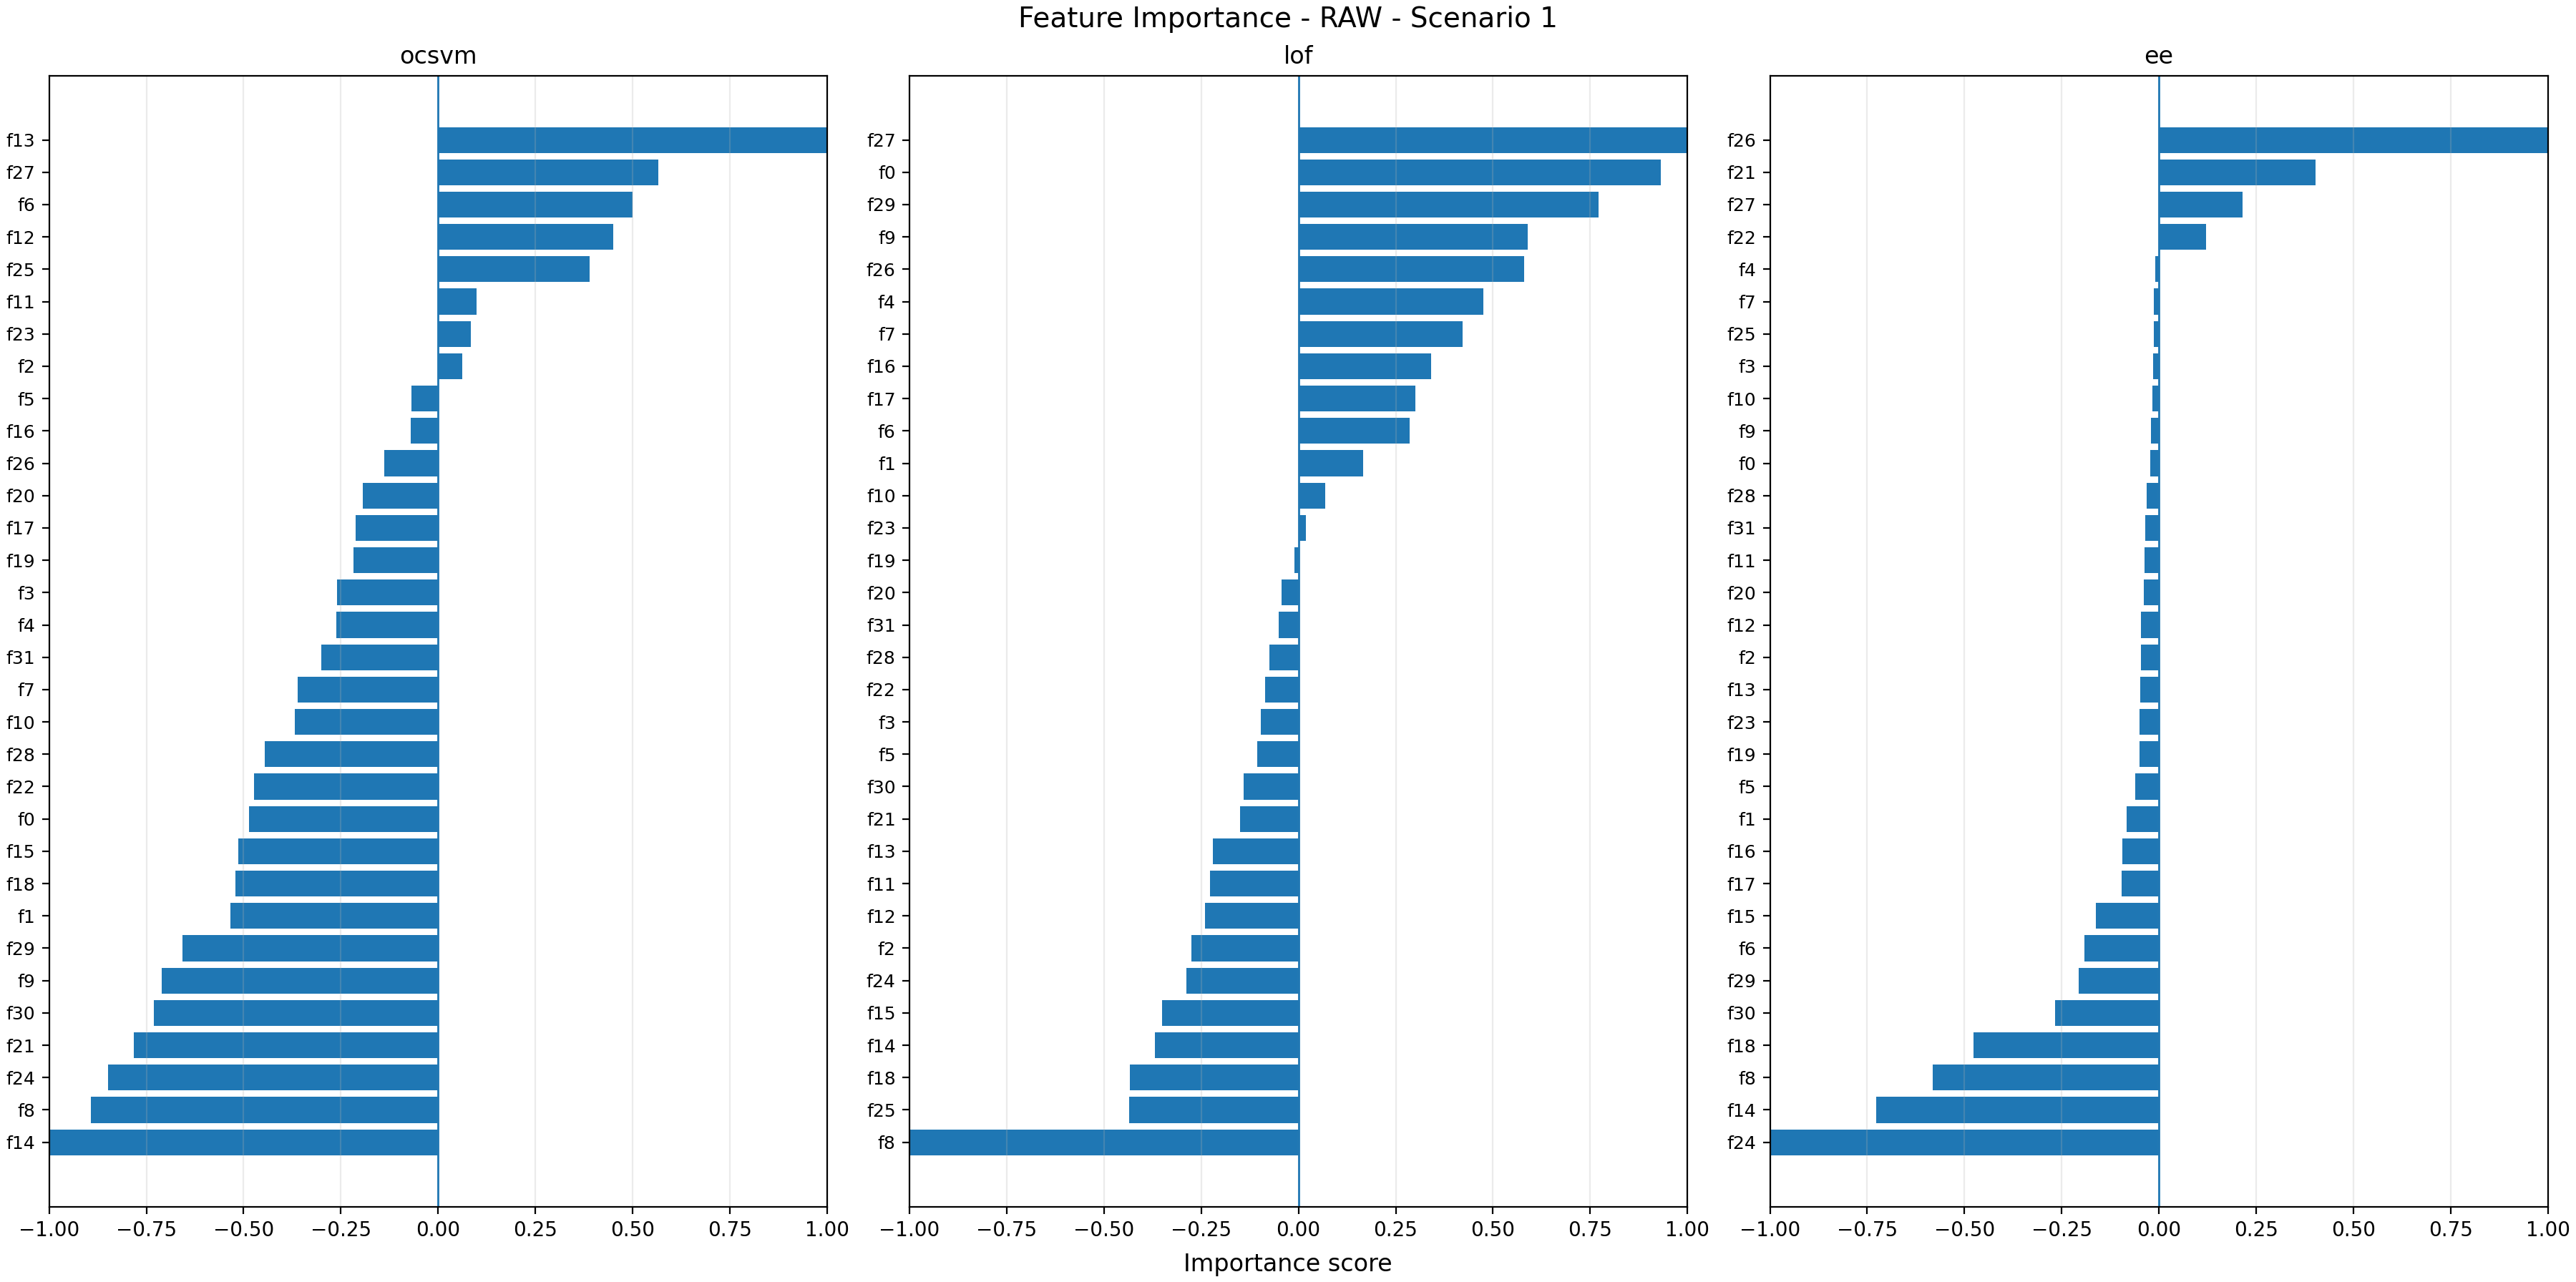
\includegraphics[width=\linewidth]{chapters/fi_helpful_panels_raw_s1.png}
	\caption{Feature Importance — RAW, Scenario 1}
	\label{fig:fi-raw-s1}
\end{figure}

For the RAW representation in Scenario~1 (see \cref{fig:fi-raw-s1}),
several consistent patterns emerge across the one-class models.
In particular, $f_{27}$ appears among the most helpful features
for all classifiers, whereas $f_{14}$ and $f_{8}$ are consistently
ranked among the most harmful.

\ac{OCSVM} and \ac{EE} rely strongly on a small number of dominant features
(\ac{OCSVM}: $f_{13}$; \ac{EE}: $f_{26}$), while \ac{LOF} distributes importance
more broadly across multiple components of the latent vector.
Furthermore, clear sign disagreements occur between classifiers,
indicating that the one-class methods extract different structural
aspects from the same feature space.

\begin{figure}[!htbp]
	\centering
	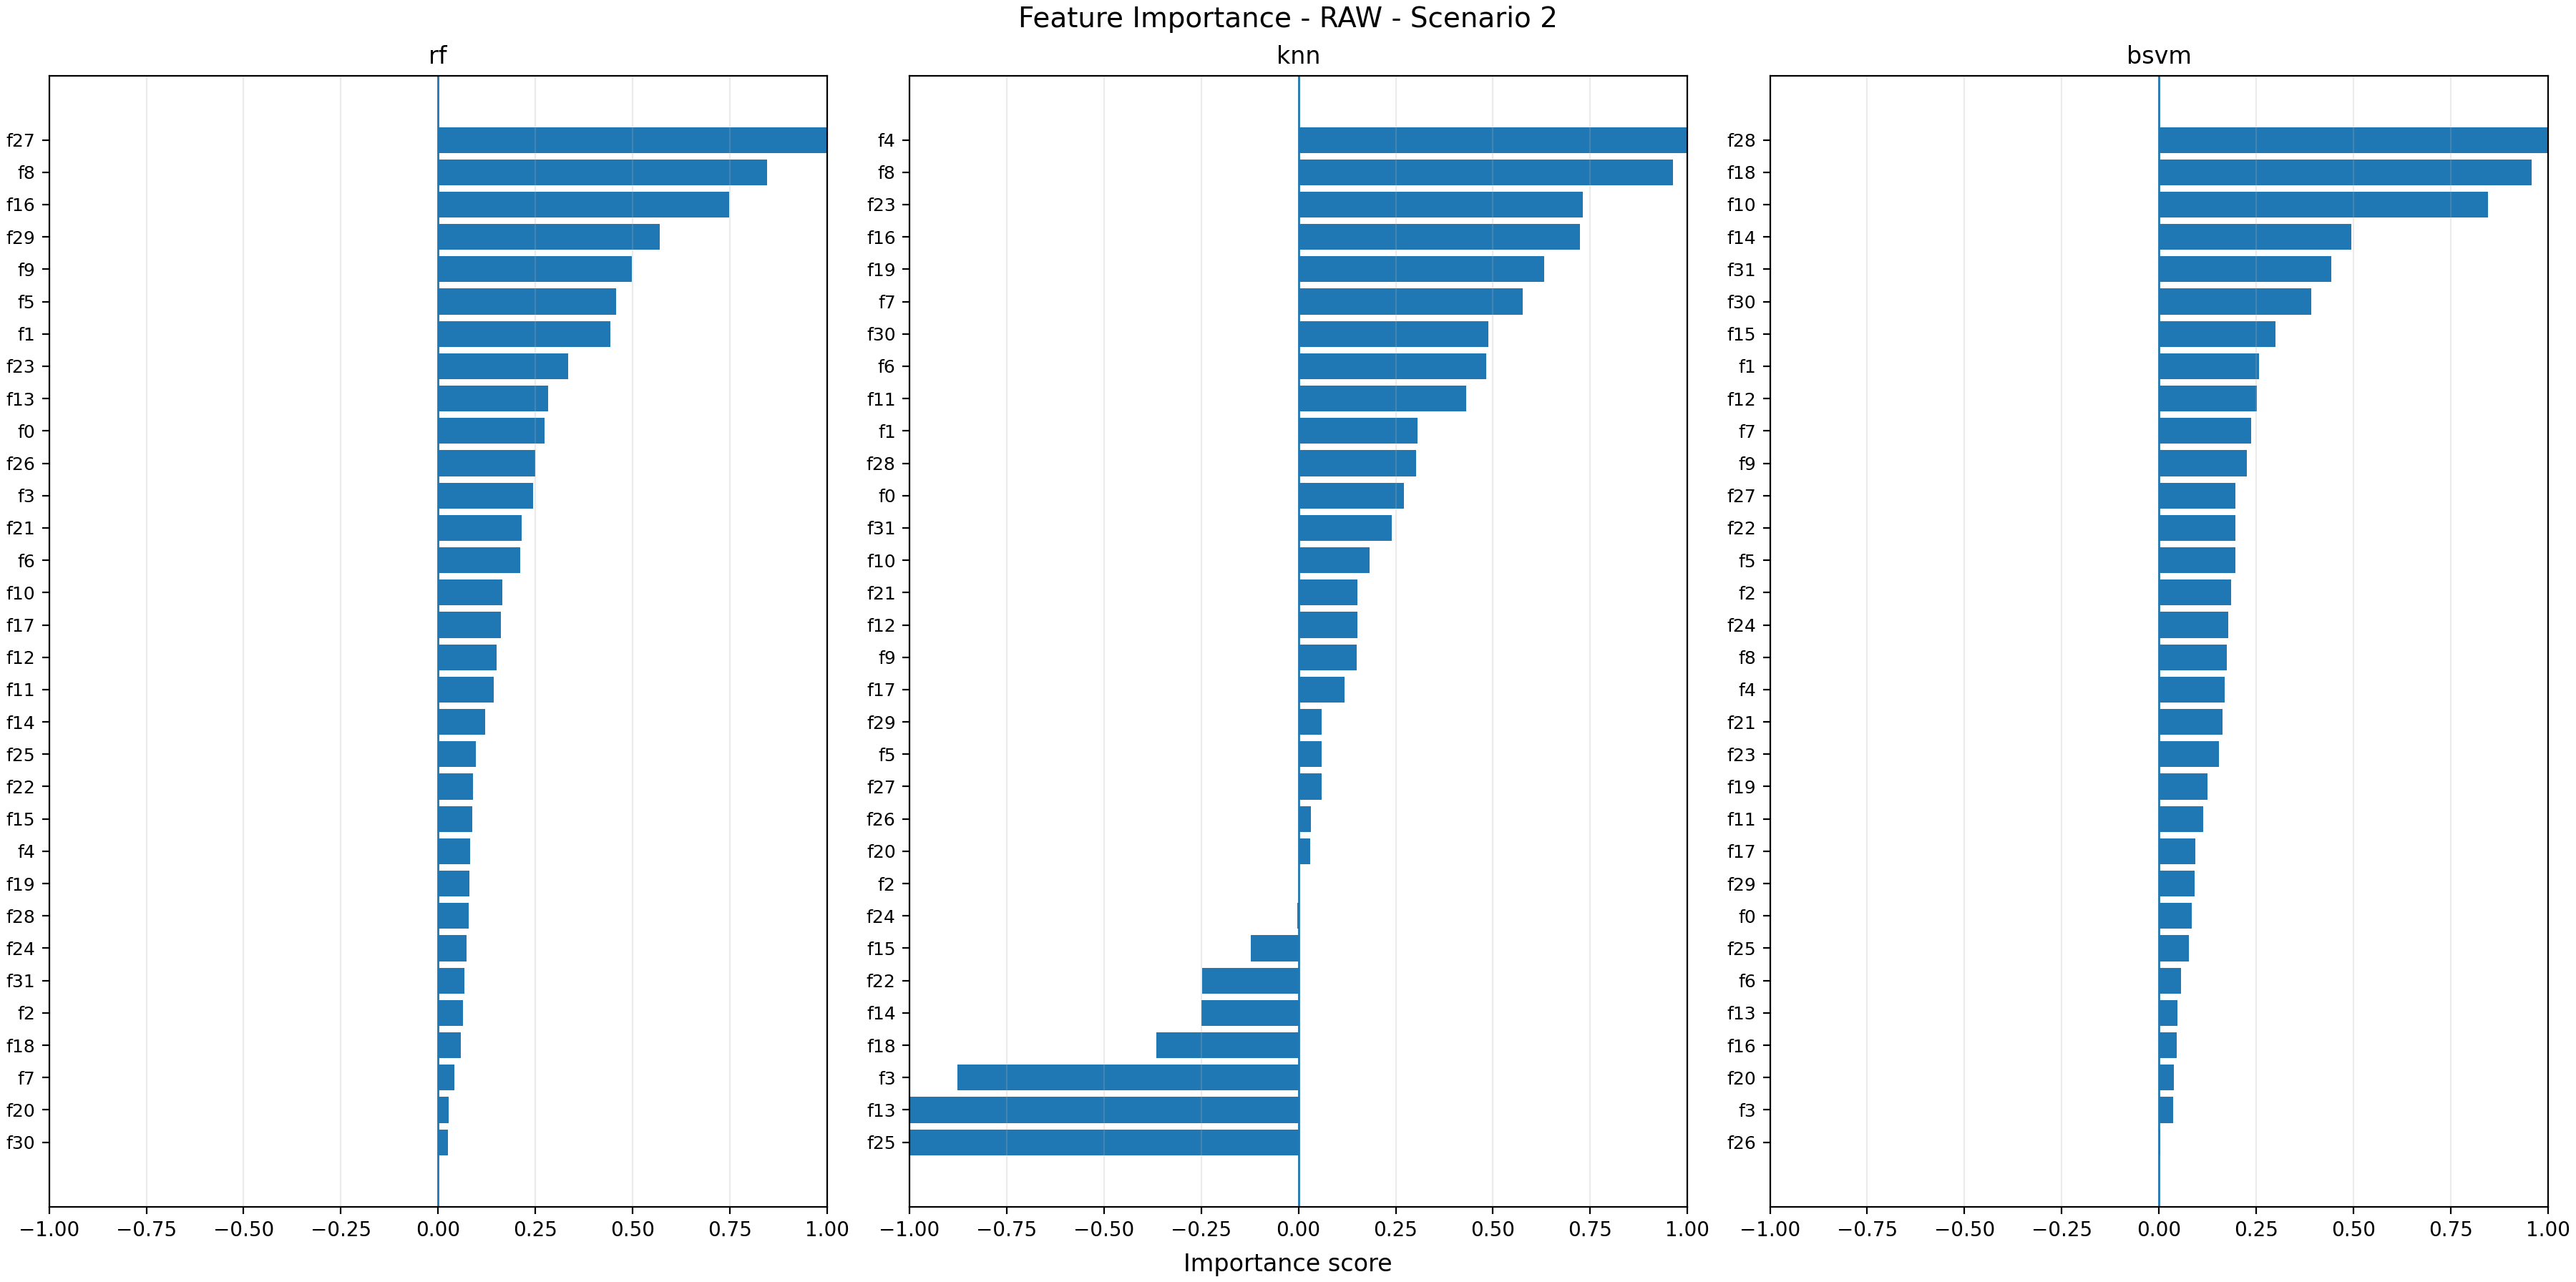
\includegraphics[width=\linewidth]{chapters/fi_helpful_panels_raw_s2.png}
	\caption{Feature Importance — RAW, Scenario 2}
	\label{fig:fi-raw-s2}
\end{figure}

In the supervised setting of Scenario~2 (\cref{fig:fi-raw-s2}),
Random Forest is dominated by a relatively small subset of features,
most prominently $f_{27}$, followed by $f_{8}$ and $f_{16}$.
\ac{KNN} exhibits a more polarized structure with both strongly positive
and strongly negative contributions, reflecting a selective reliance
on specific latent dimensions.

Binary \ac{SVM} emphasizes a partially different subset of features,
suggesting that the linear decision boundary captures directions
in the latent space that differ from those exploited by tree-based
or neighbor-based models.

\begin{figure}[!htbp]
	\centering
	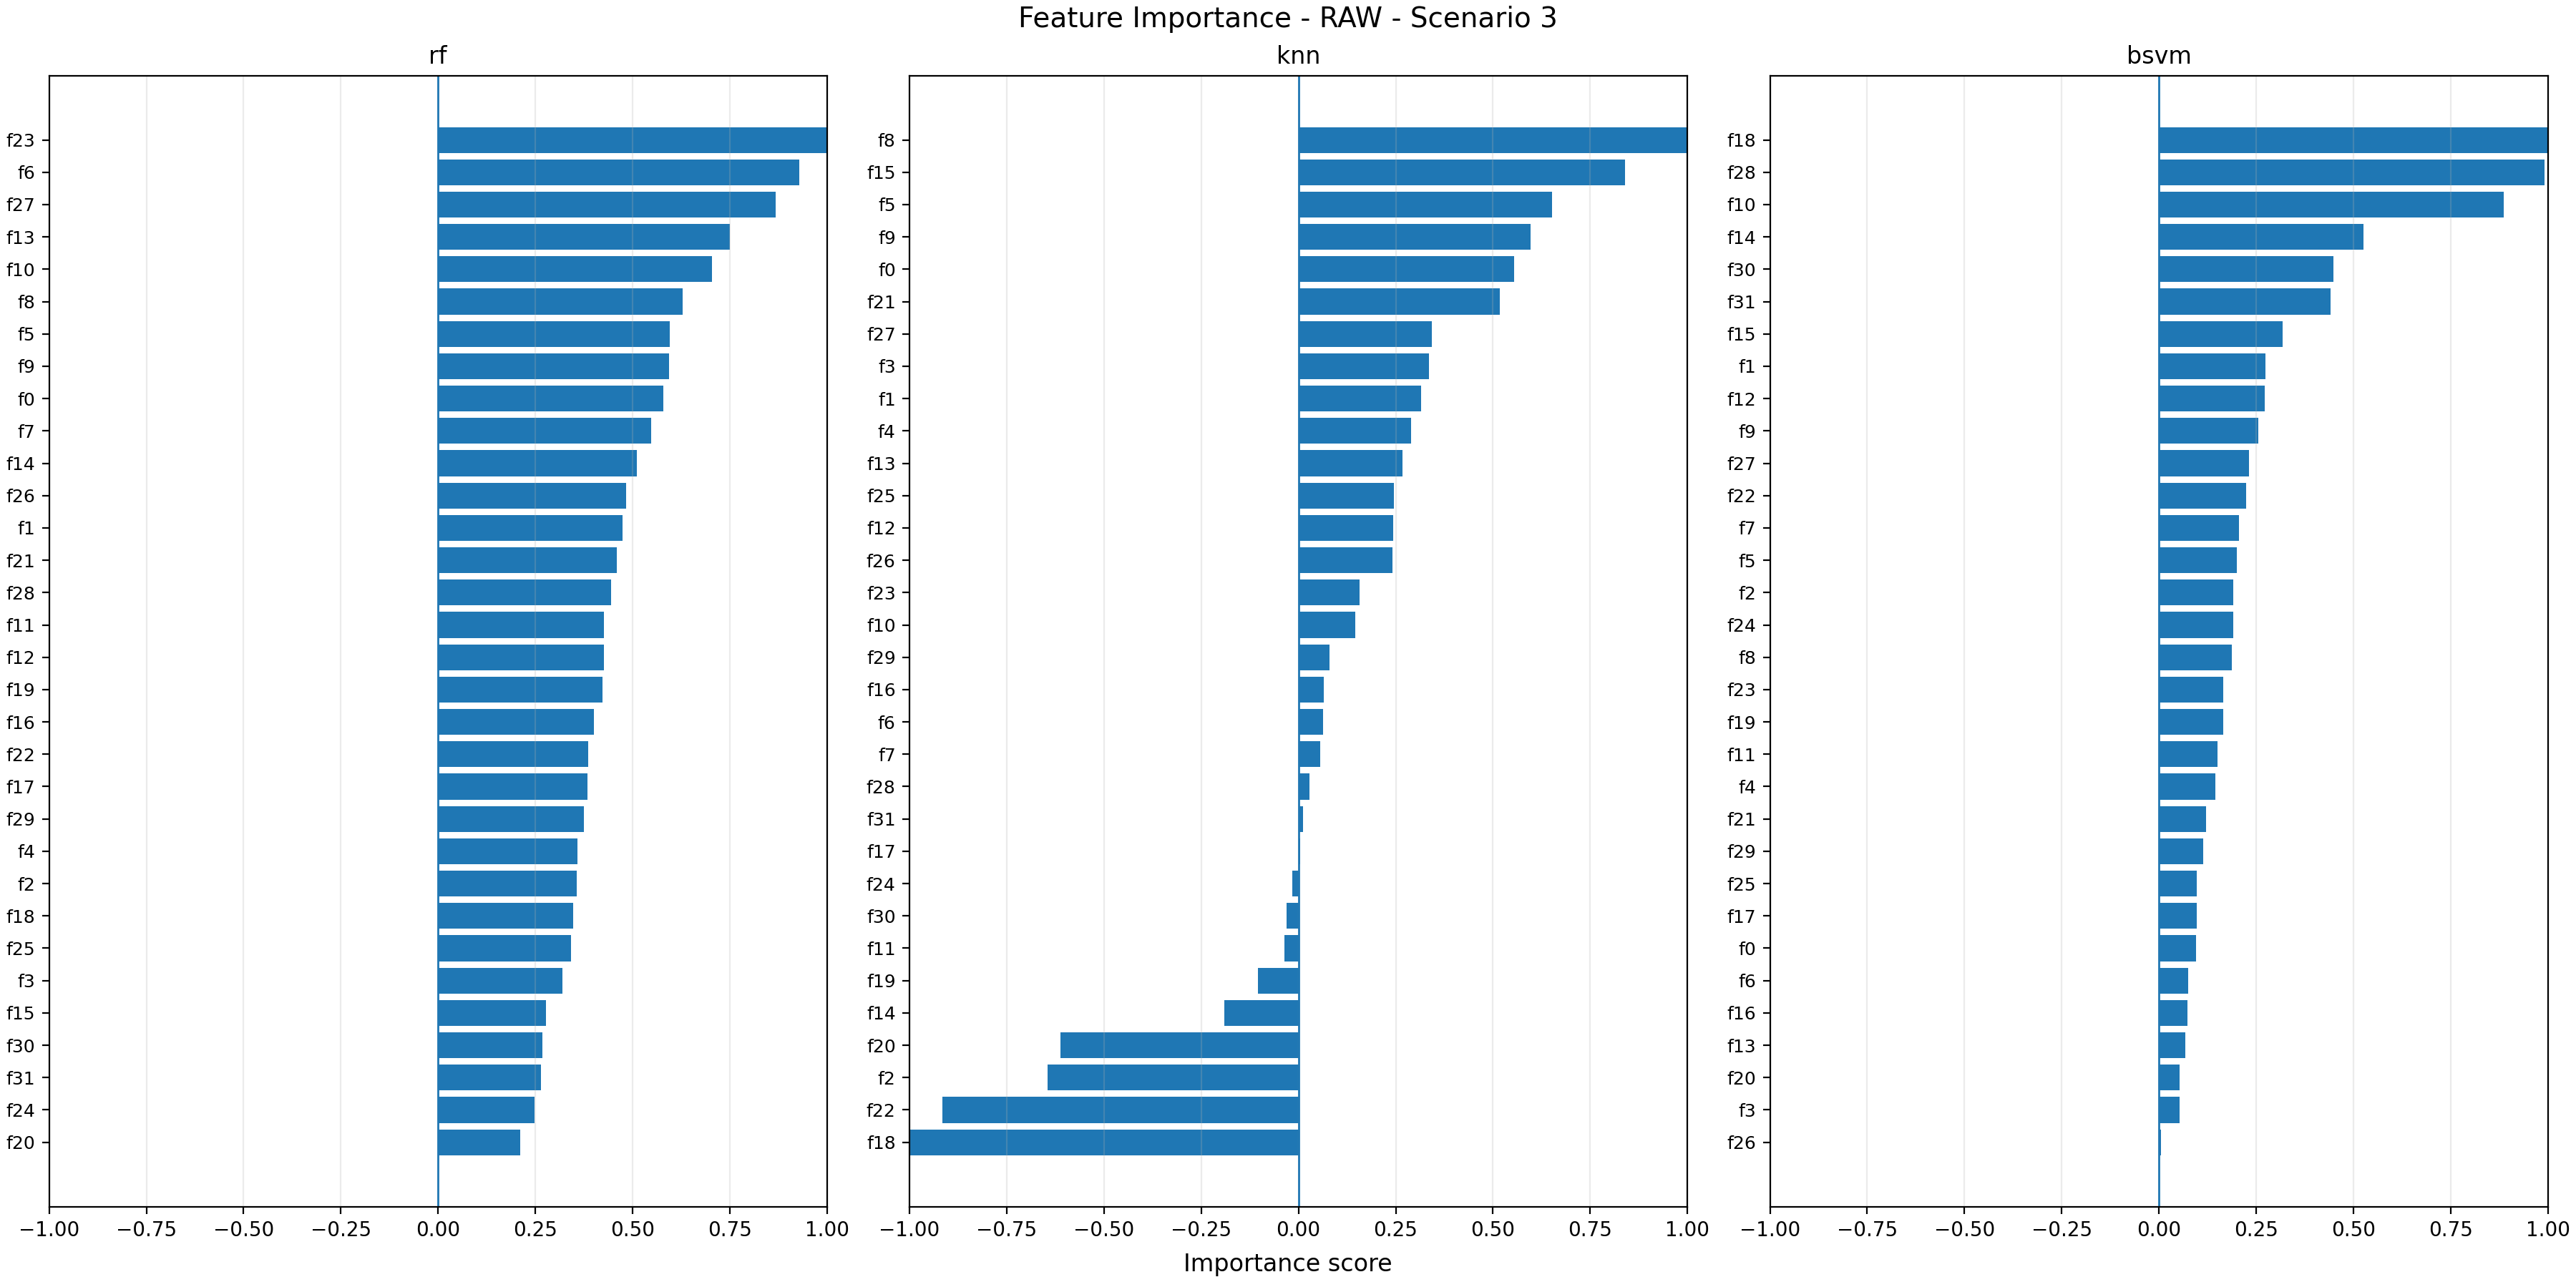
\includegraphics[width=\linewidth]{chapters/fi_helpful_panels_raw_s3.png}
	\caption{Feature Importance — RAW, Scenario 3}
	\label{fig:fi-raw-s3}
\end{figure}
\clearpage

Under the more challenging generalization setting of Scenario~3
(\cref{fig:fi-raw-s3}), importance patterns become more concentrated.
Random Forest highlights a compact group of dominant features,
while \ac{KNN} again shows strong positive and negative contributions.
Binary \ac{SVM} focuses on a limited subset of high-weight components.

Notably, certain features such as $f_{27}$ and $f_{8}$ remain
consistently relevant across classifiers, indicating that specific
latent dimensions retain discriminative power even when attack
types differ between training and testing.

\begin{figure}[!htbp]
	\centering
	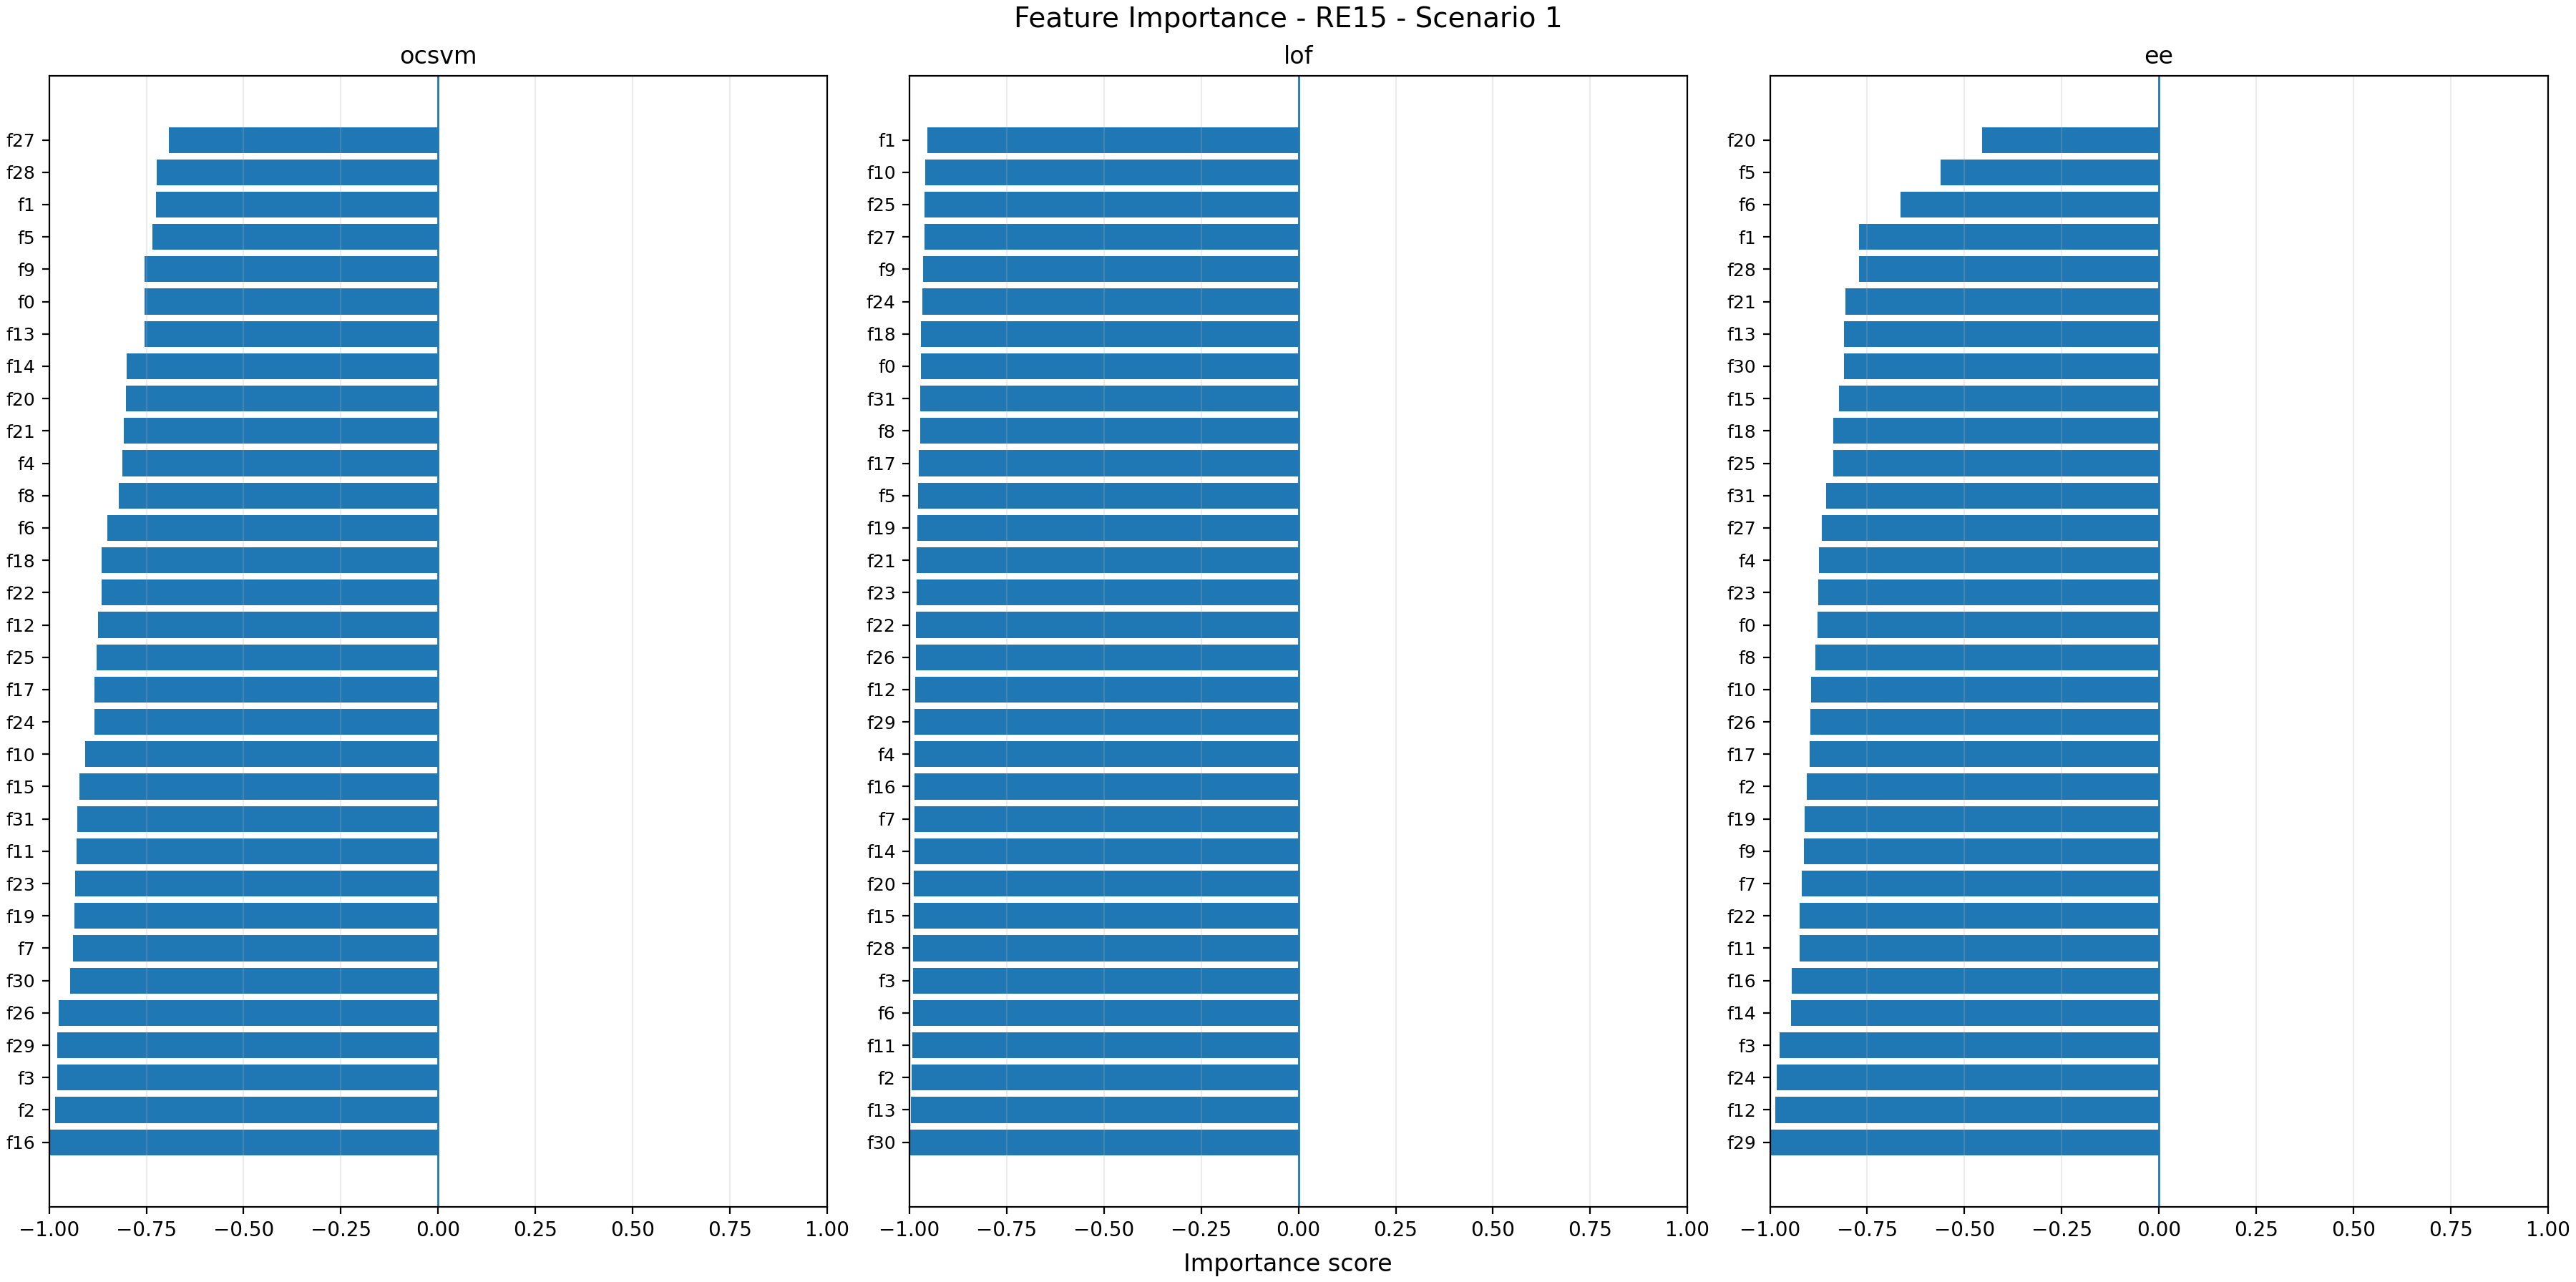
\includegraphics[width=\linewidth]{chapters/fi_helpful_panels_re15_s1.png}
	\caption{Feature Importance — RE15, Scenario 1}
	\label{fig:fi-re15-s1}
\end{figure}

For the RE15 representation in Scenario~1
(\cref{fig:fi-re15-s1}), the pattern differs markedly from RAW.
Nearly all features receive negative importance values across
classifiers, and no clearly beneficial subset emerges.
This indicates that the reverse-engineered representation does not
provide strong discriminative structure for one-class detection
in this configuration.

\begin{figure}[!htbp]
	\centering
	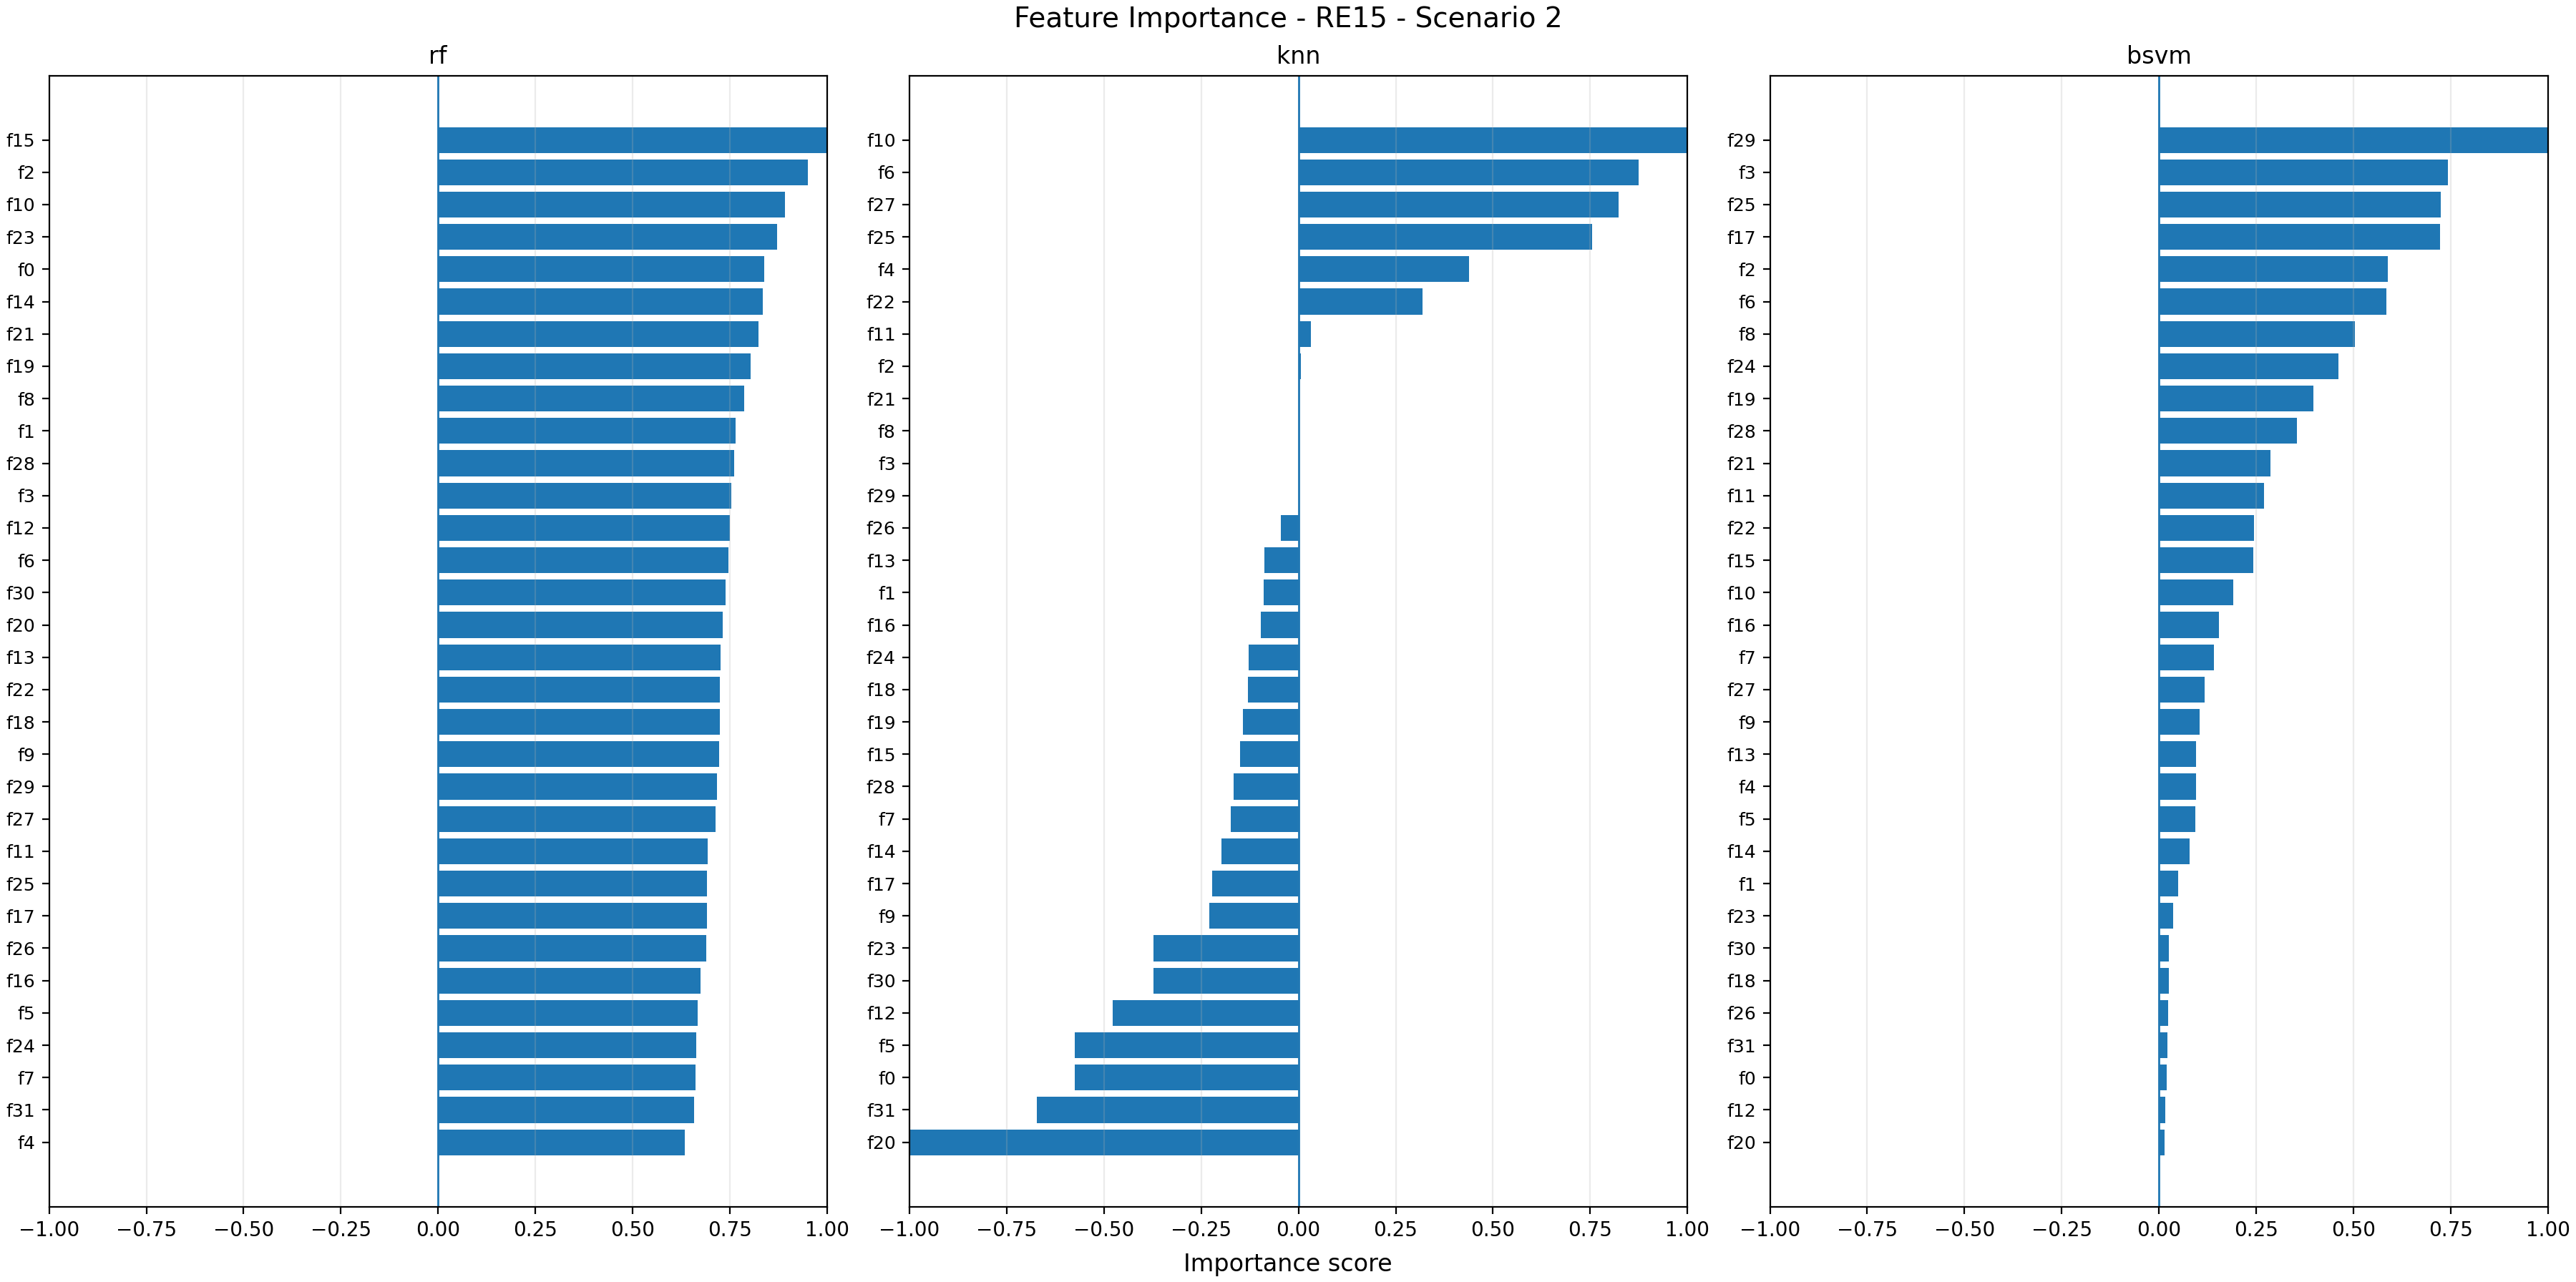
\includegraphics[width=\linewidth]{chapters/fi_helpful_panels_re15_s2.png}
	\caption{Feature Importance — RE15, Scenario 2}
	\label{fig:fi-re15-s2}
\end{figure}

In Scenario~2 with RE15 (\cref{fig:fi-re15-s2}), the classifiers
exhibit more differentiated behavior.
Random Forest distributes importance relatively broadly,
\ac{KNN} again separates helpful from harmful features,
and Binary \ac{SVM} concentrates on a smaller subset of dominant weights.

Although limited cross-model overlap exists (e.g., $f_{10}$ appears
relevant for multiple classifiers), overall agreement between models
is weaker than observed for the RAW representation.

\begin{figure}[!htbp]
	\centering
	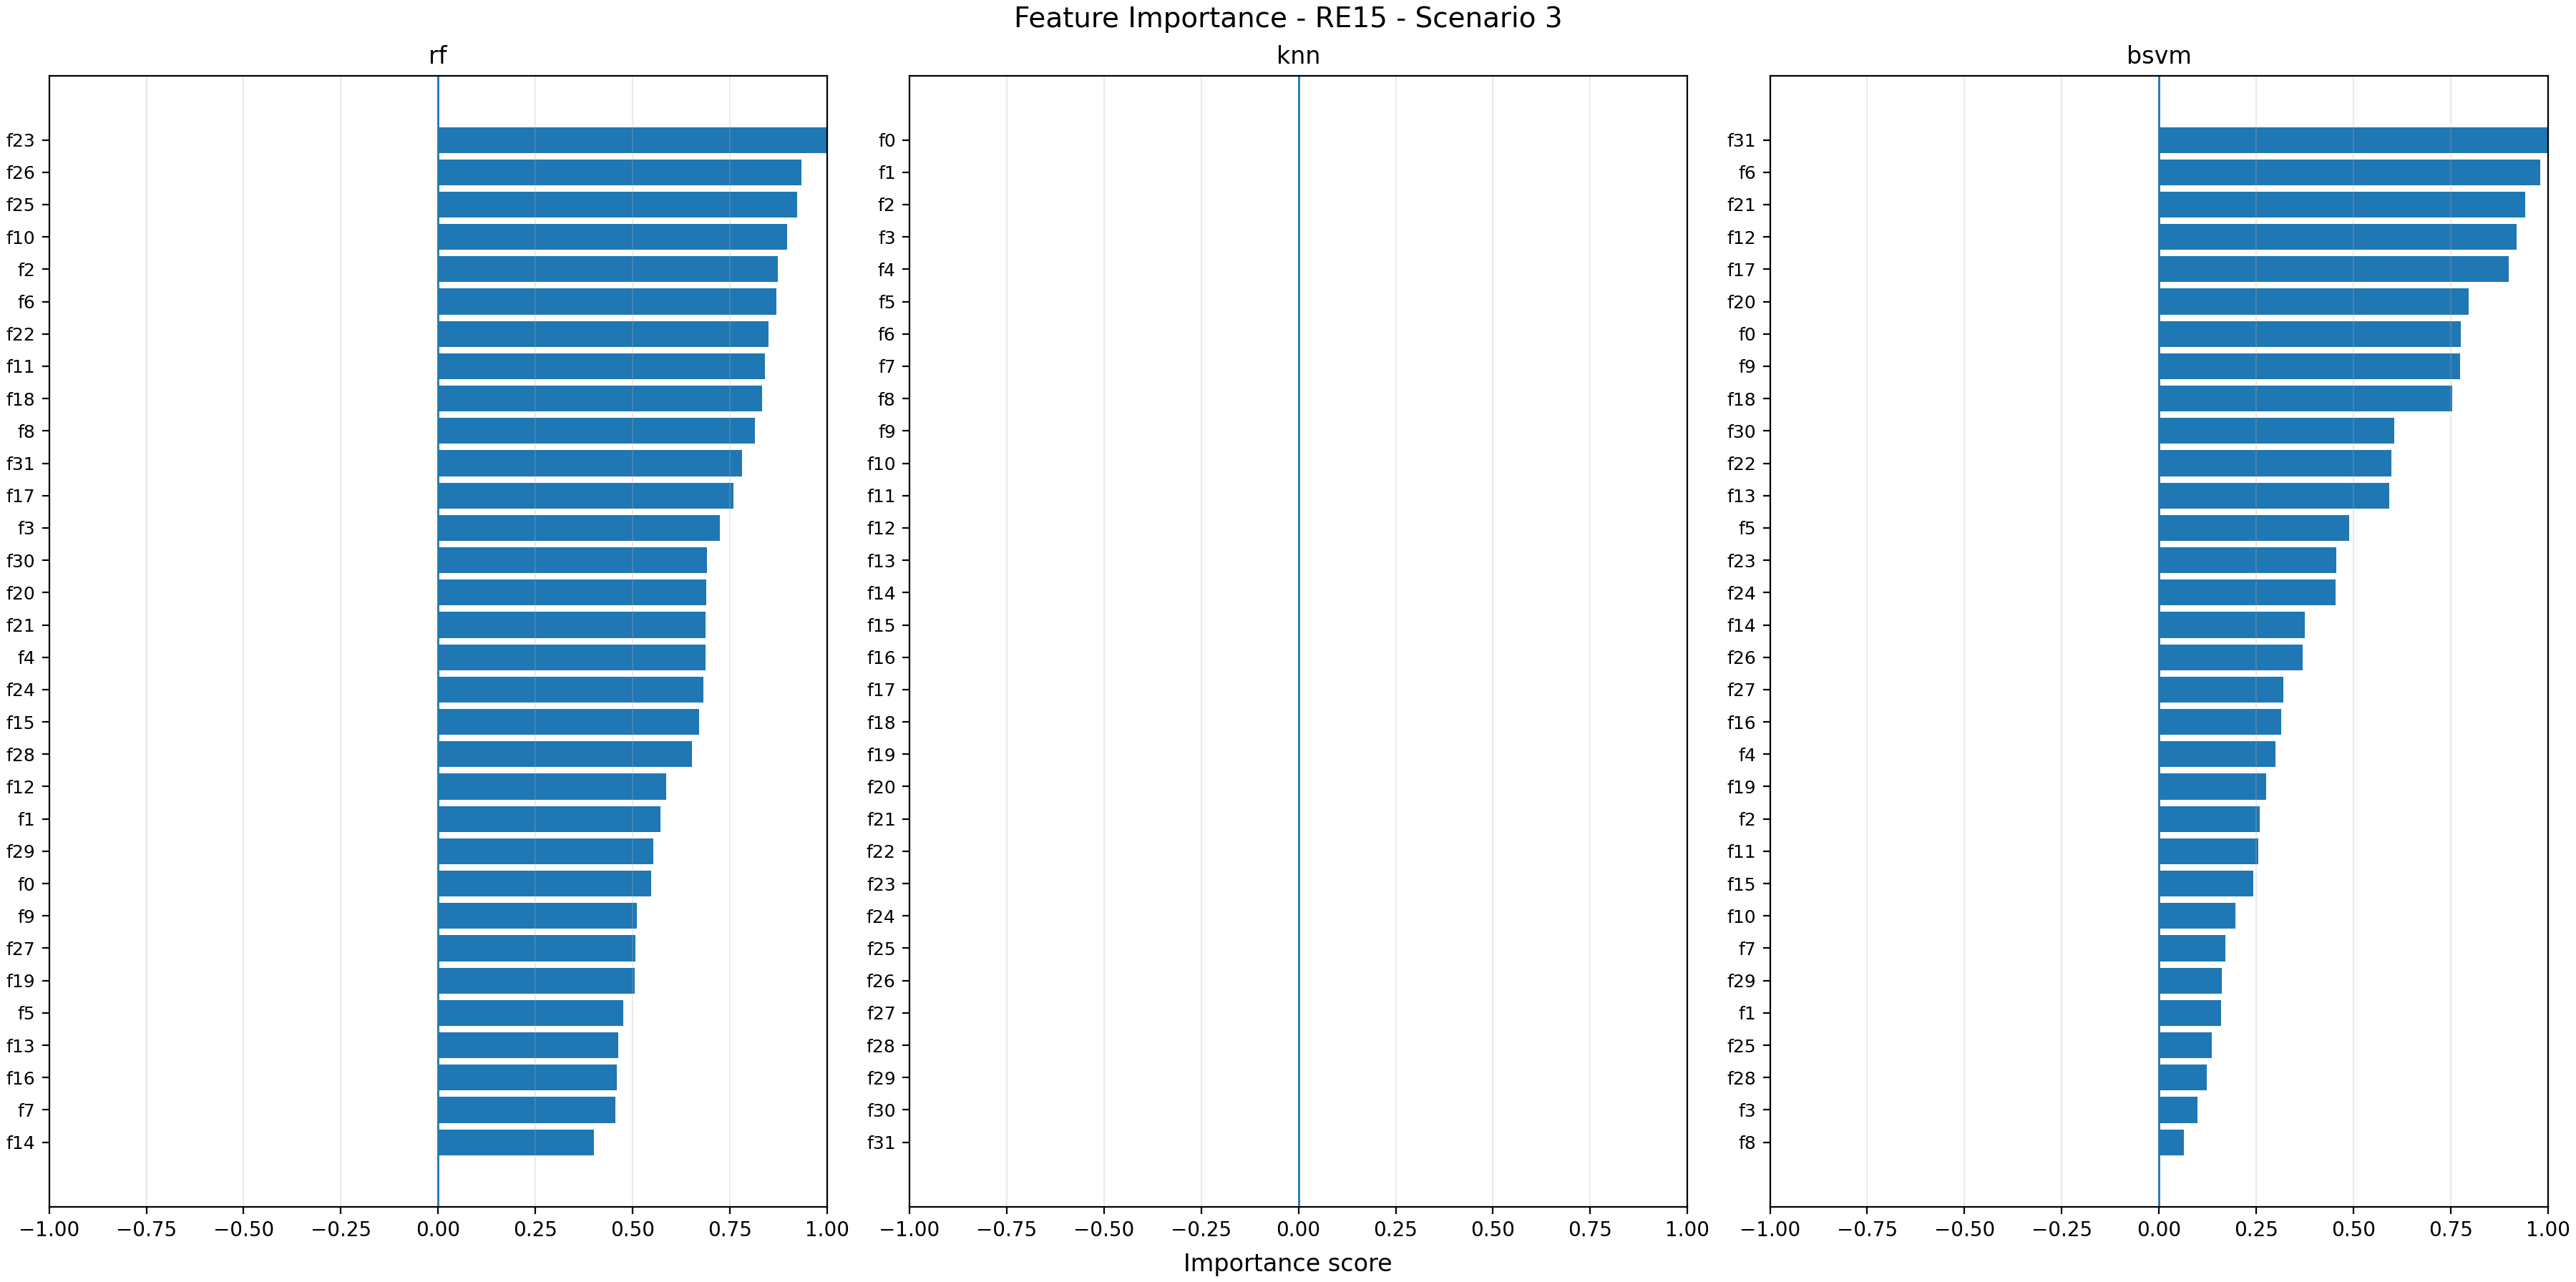
\includegraphics[width=\linewidth]{chapters/fi_helpful_panels_re15_s3.png}
	\caption{Feature Importance — RE15, Scenario 3}
	\label{fig:fi-re15-s3}
\end{figure}

In Scenario~3 under RE15 (\cref{fig:fi-re15-s3}),
the importance structure becomes considerably less distinctive.
\ac{KNN} assigns nearly uniform importance across features,
Random Forest distributes importance broadly without clear dominance,
and Binary \ac{SVM} concentrates on a small subset of higher-weight
components.

Overall, the RE15 representation yields less structured and less
consistent importance patterns than RAW, which aligns with the
observed degradation in classification performance.

\clearpage
\subsection{Venn Diagrams}

The Venn diagrams visualize the overlap of misclassified samples
between the three traditional \ac{ML} classifiers within each scenario.
Each circle represents the set of incorrectly classified instances
for one classifier. Pairwise intersections indicate samples that
are misclassified by two classifiers, while the triple intersection
represents instances that are misclassified by all three models.
Large overlap regions therefore indicate agreement in error behavior,
whereas large regions without overlaps reveal classifier-specific weaknesses.

\begin{figure}[!htbp]
    \centering
    \begin{subfigure}[t]{0.32\linewidth}
        \centering
        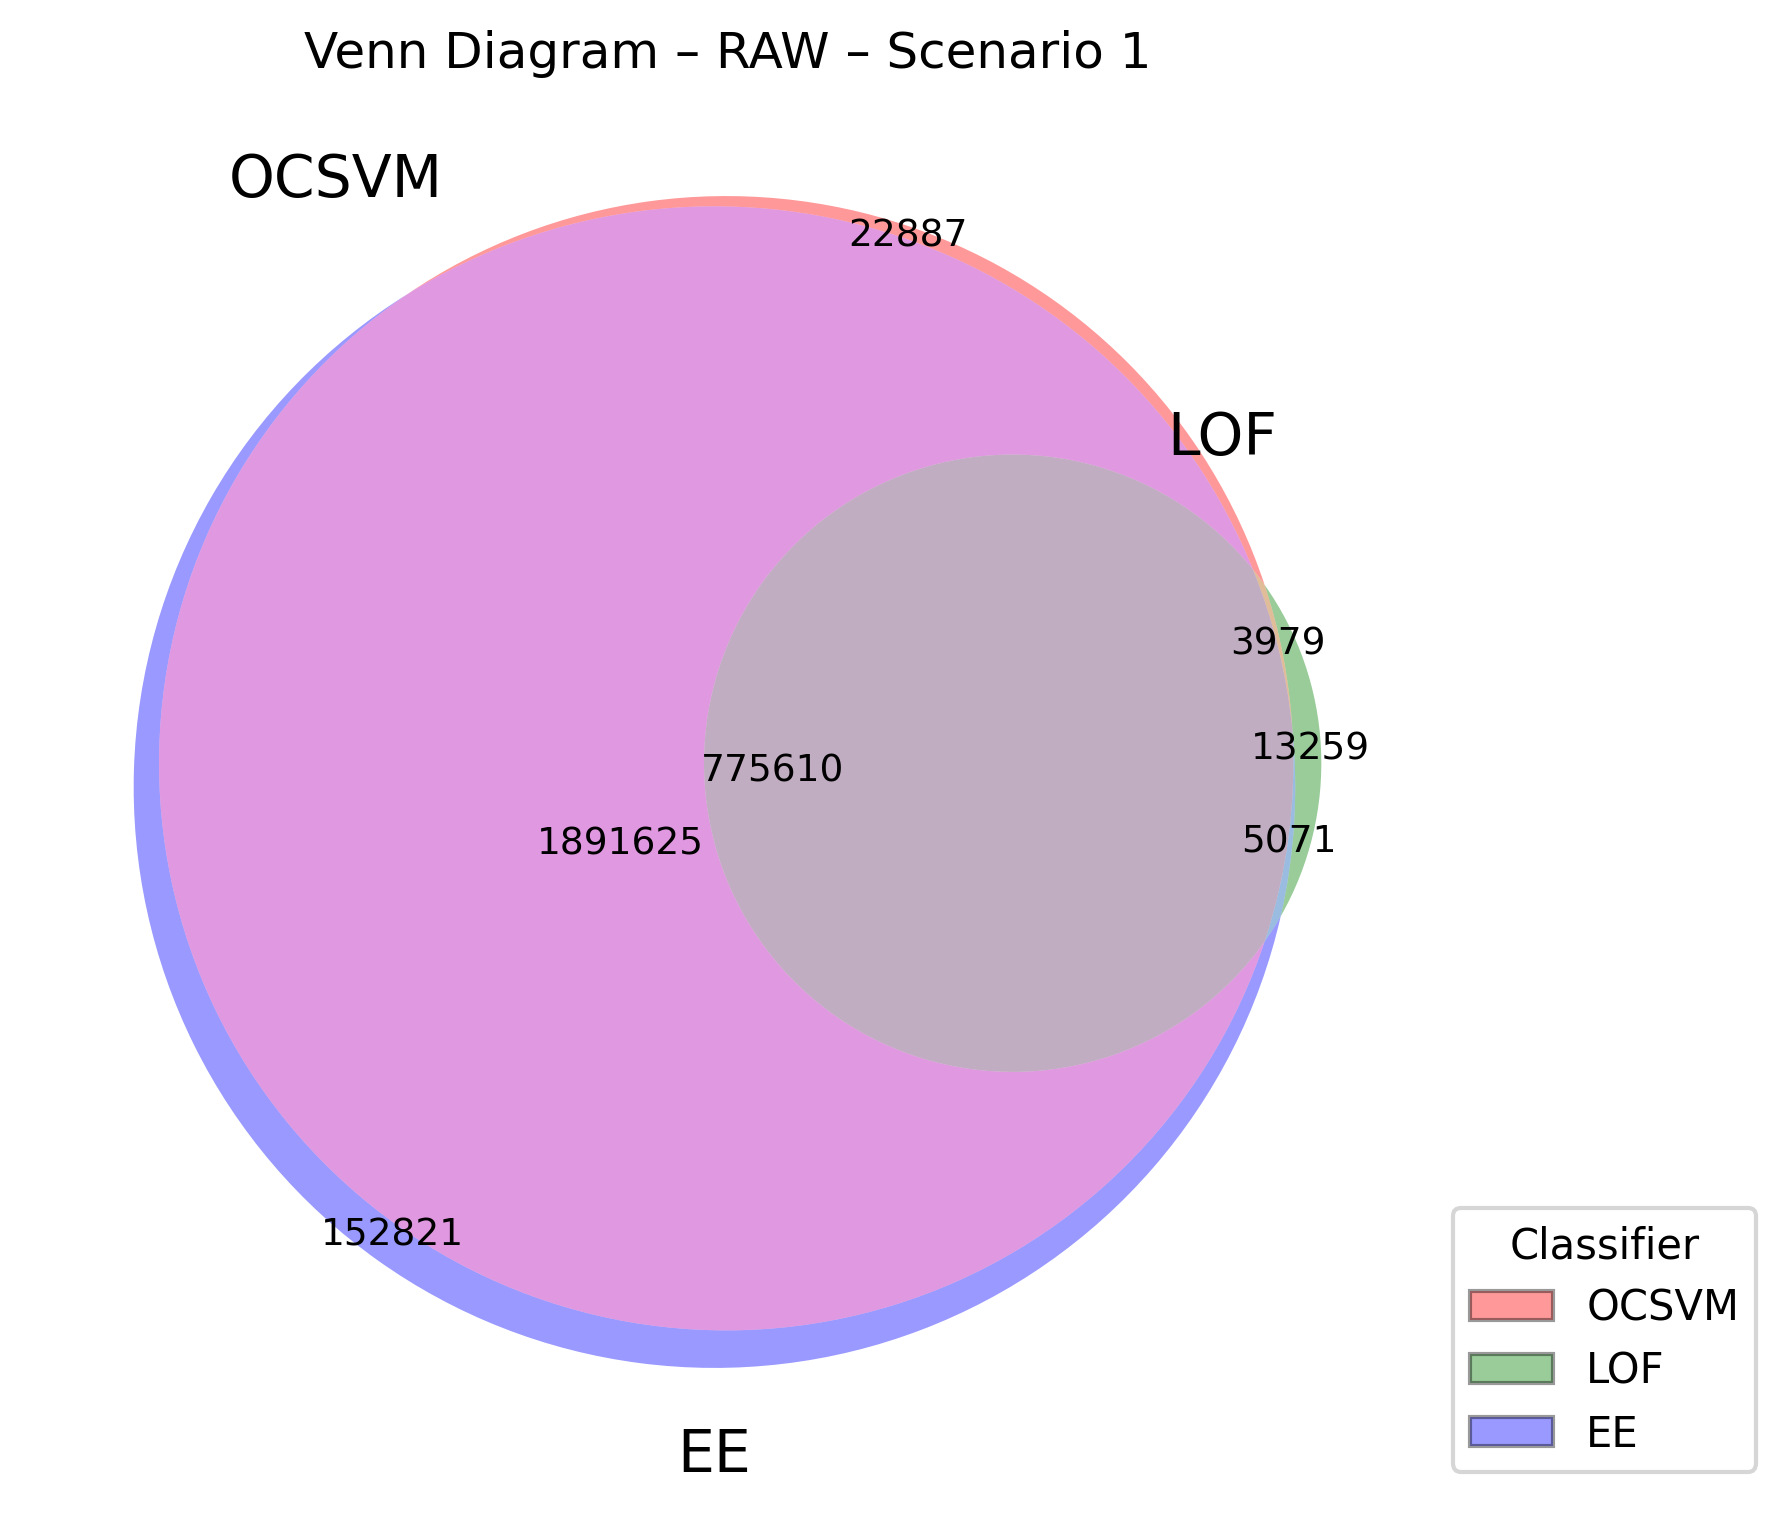
\includegraphics[width=\linewidth]{chapters/venn_raw_s1.png}
        \caption{Scenario 1}
    \end{subfigure}\hfill
    \begin{subfigure}[t]{0.32\linewidth}
        \centering
        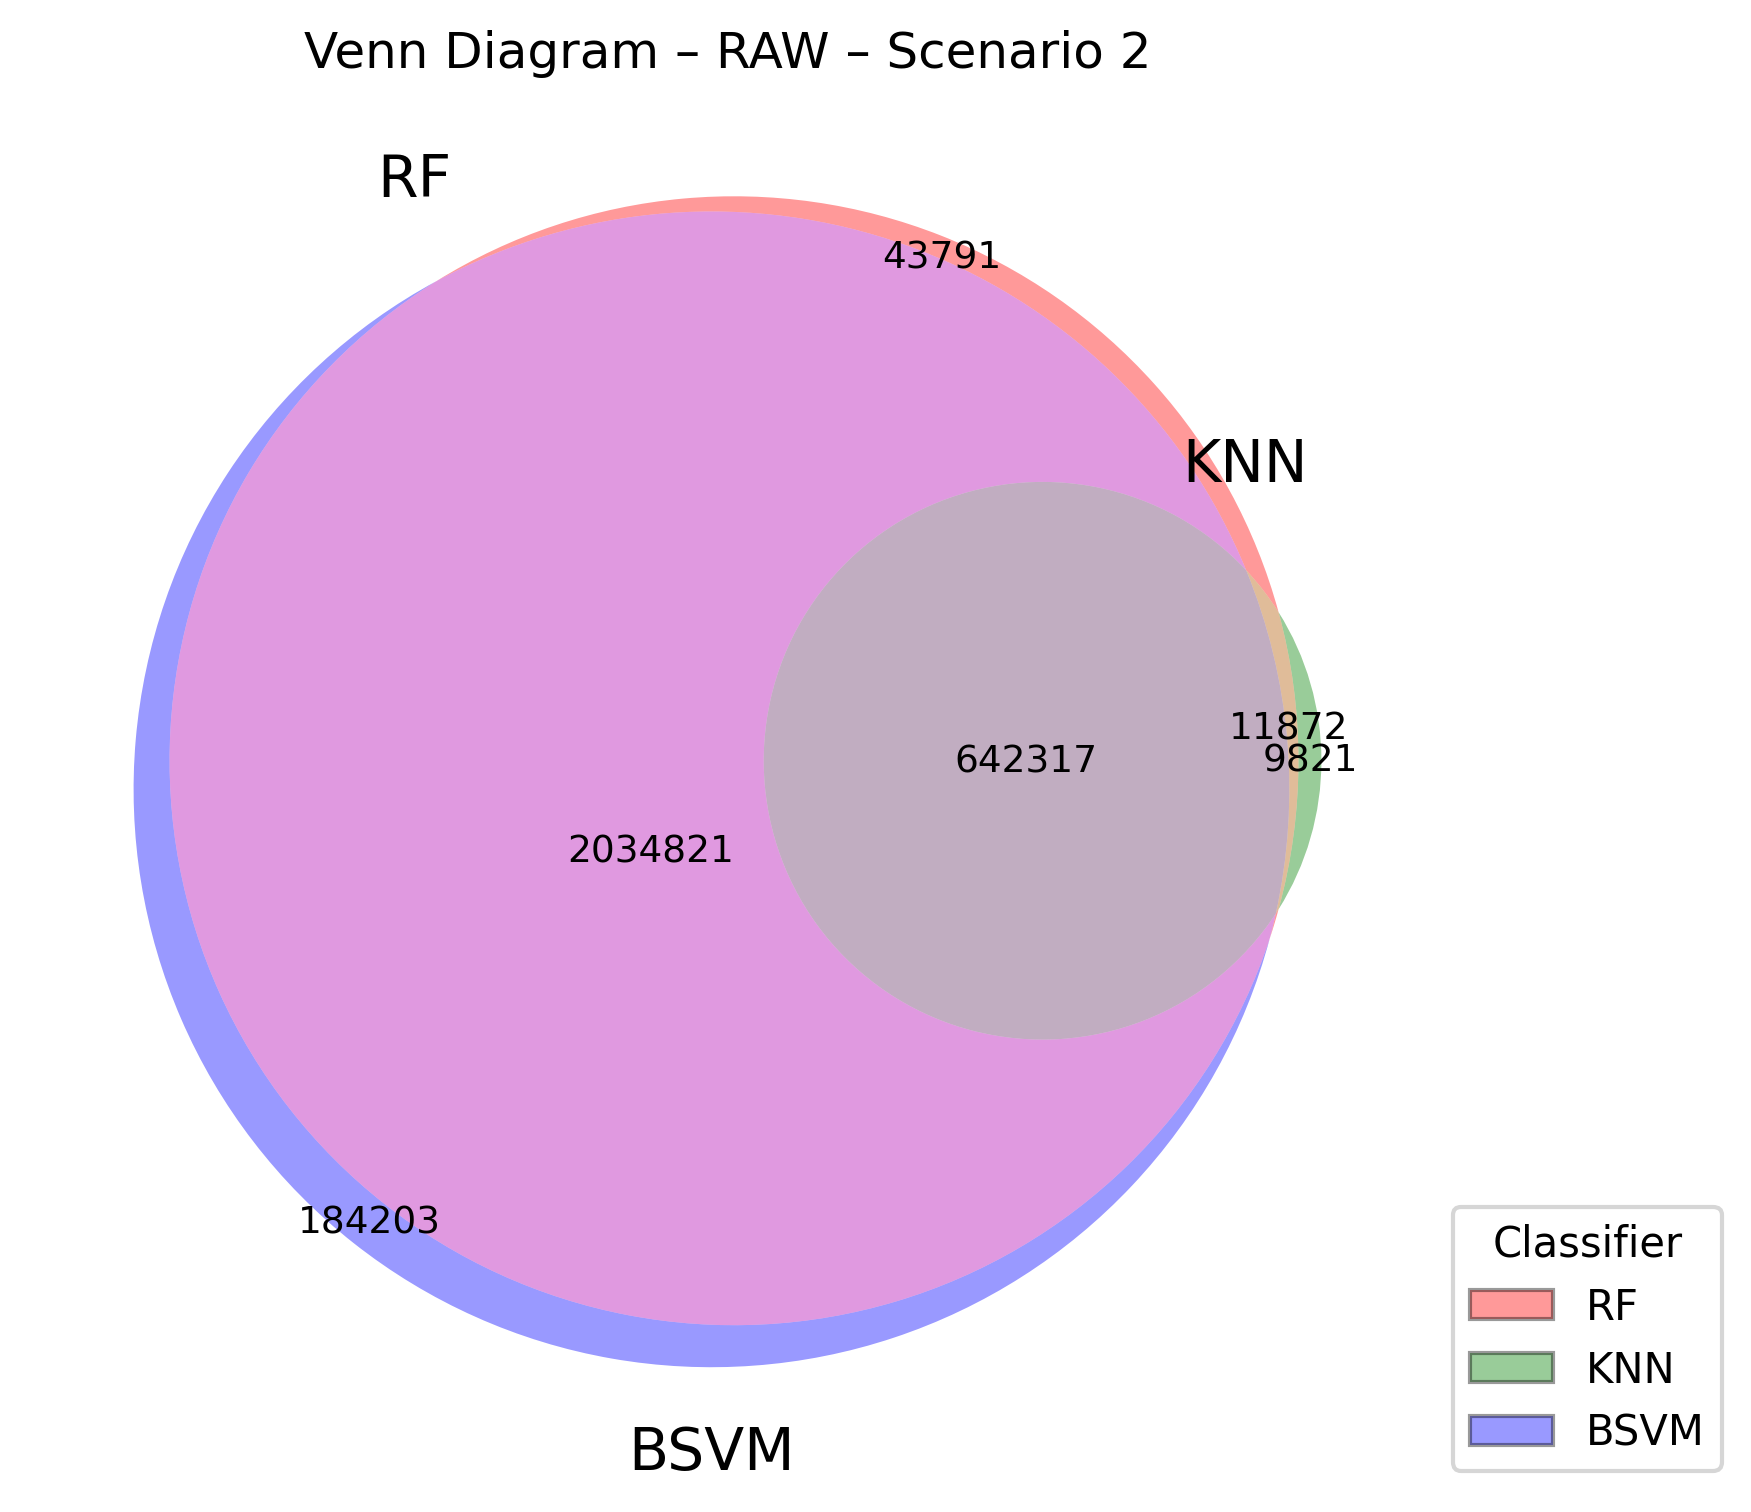
\includegraphics[width=\linewidth]{chapters/venn_raw_s2.png}
        \caption{Scenario 2}
    \end{subfigure}\hfill
    \begin{subfigure}[t]{0.32\linewidth}
        \centering
        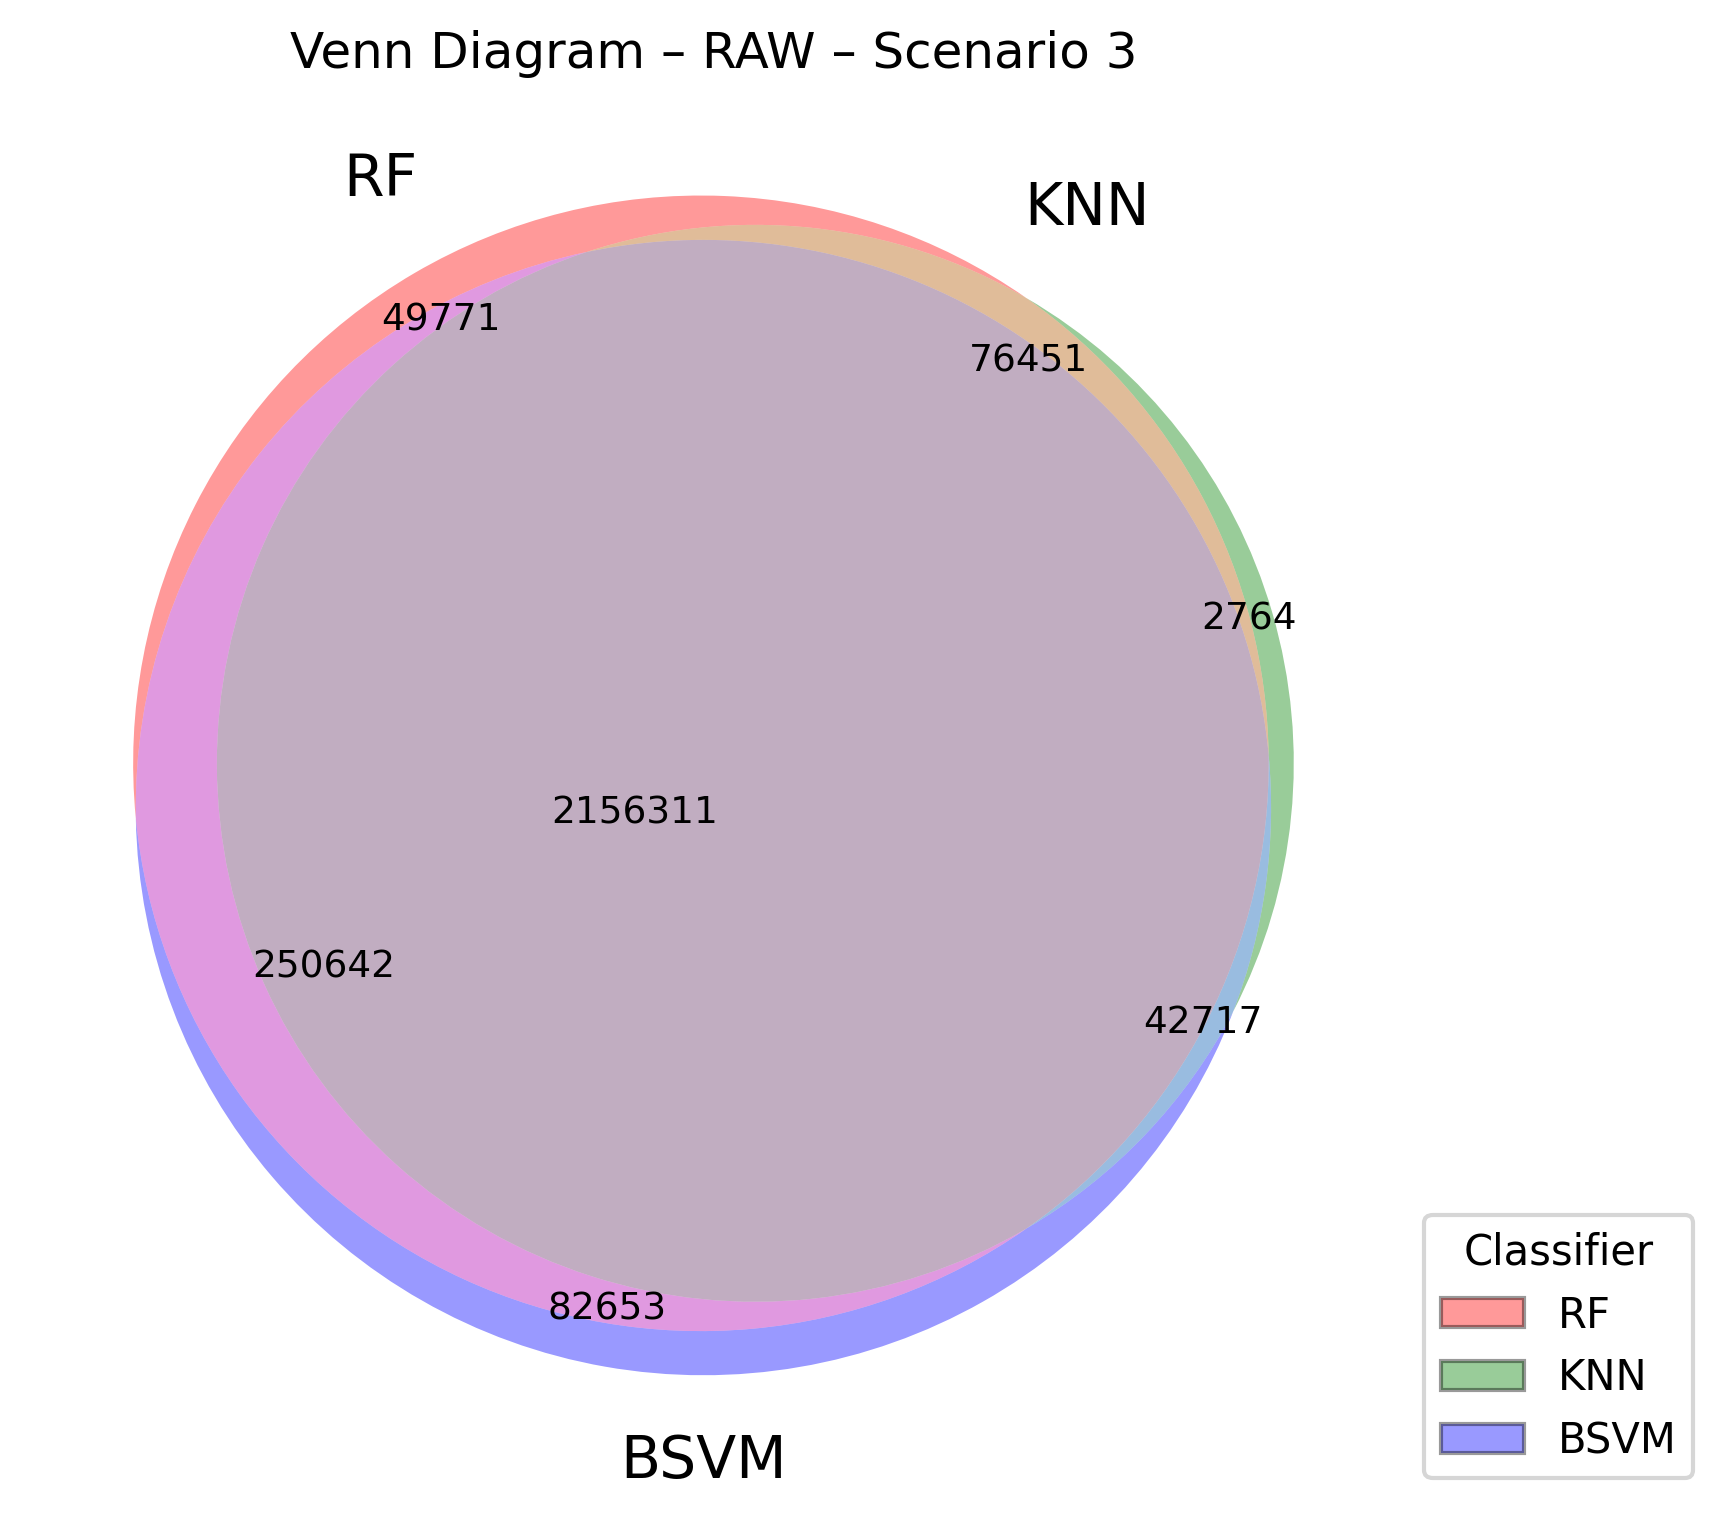
\includegraphics[width=\linewidth]{chapters/venn_raw_s3.png}
        \caption{Scenario 3}
    \end{subfigure}
    \caption{Error overlaps (Venn diagrams) for the RAW representation.}
    \label{fig:venn-raw}
\end{figure}

\paragraph{RAW Representation}

For the RAW dataset, the absolute number of errors is substantially
higher due to the larger number of evaluated samples. As \cref{fig:venn-raw} shows in Scenarios~1
and~2, the diagrams are dominated by large pairwise overlaps.
In particular, OCSVM and EE (Scenario~1) as well as RF and Binary SVM
(Scenario~2) exhibit highly similar error patterns. This suggests that
these classifier pairs learn comparable decision boundaries when using
RAW packet features, while the third classifier contributes only a
limited amount of additional unique errors.

In Scenario~3 (RAW), the triple intersection becomes the dominant
region. Most misclassified instances are shared across all classifiers,
indicating that errors are not model-specific but correspond to a
common subset of intrinsically difficult samples. This observation
explains why ensemble aggregation provides only limited improvement
in this scenario: when all base classifiers fail on the same instances,
the ensemble cannot compensate.

\begin{figure}[!htbp]
    \centering
    \begin{subfigure}[t]{0.32\linewidth}
        \centering
        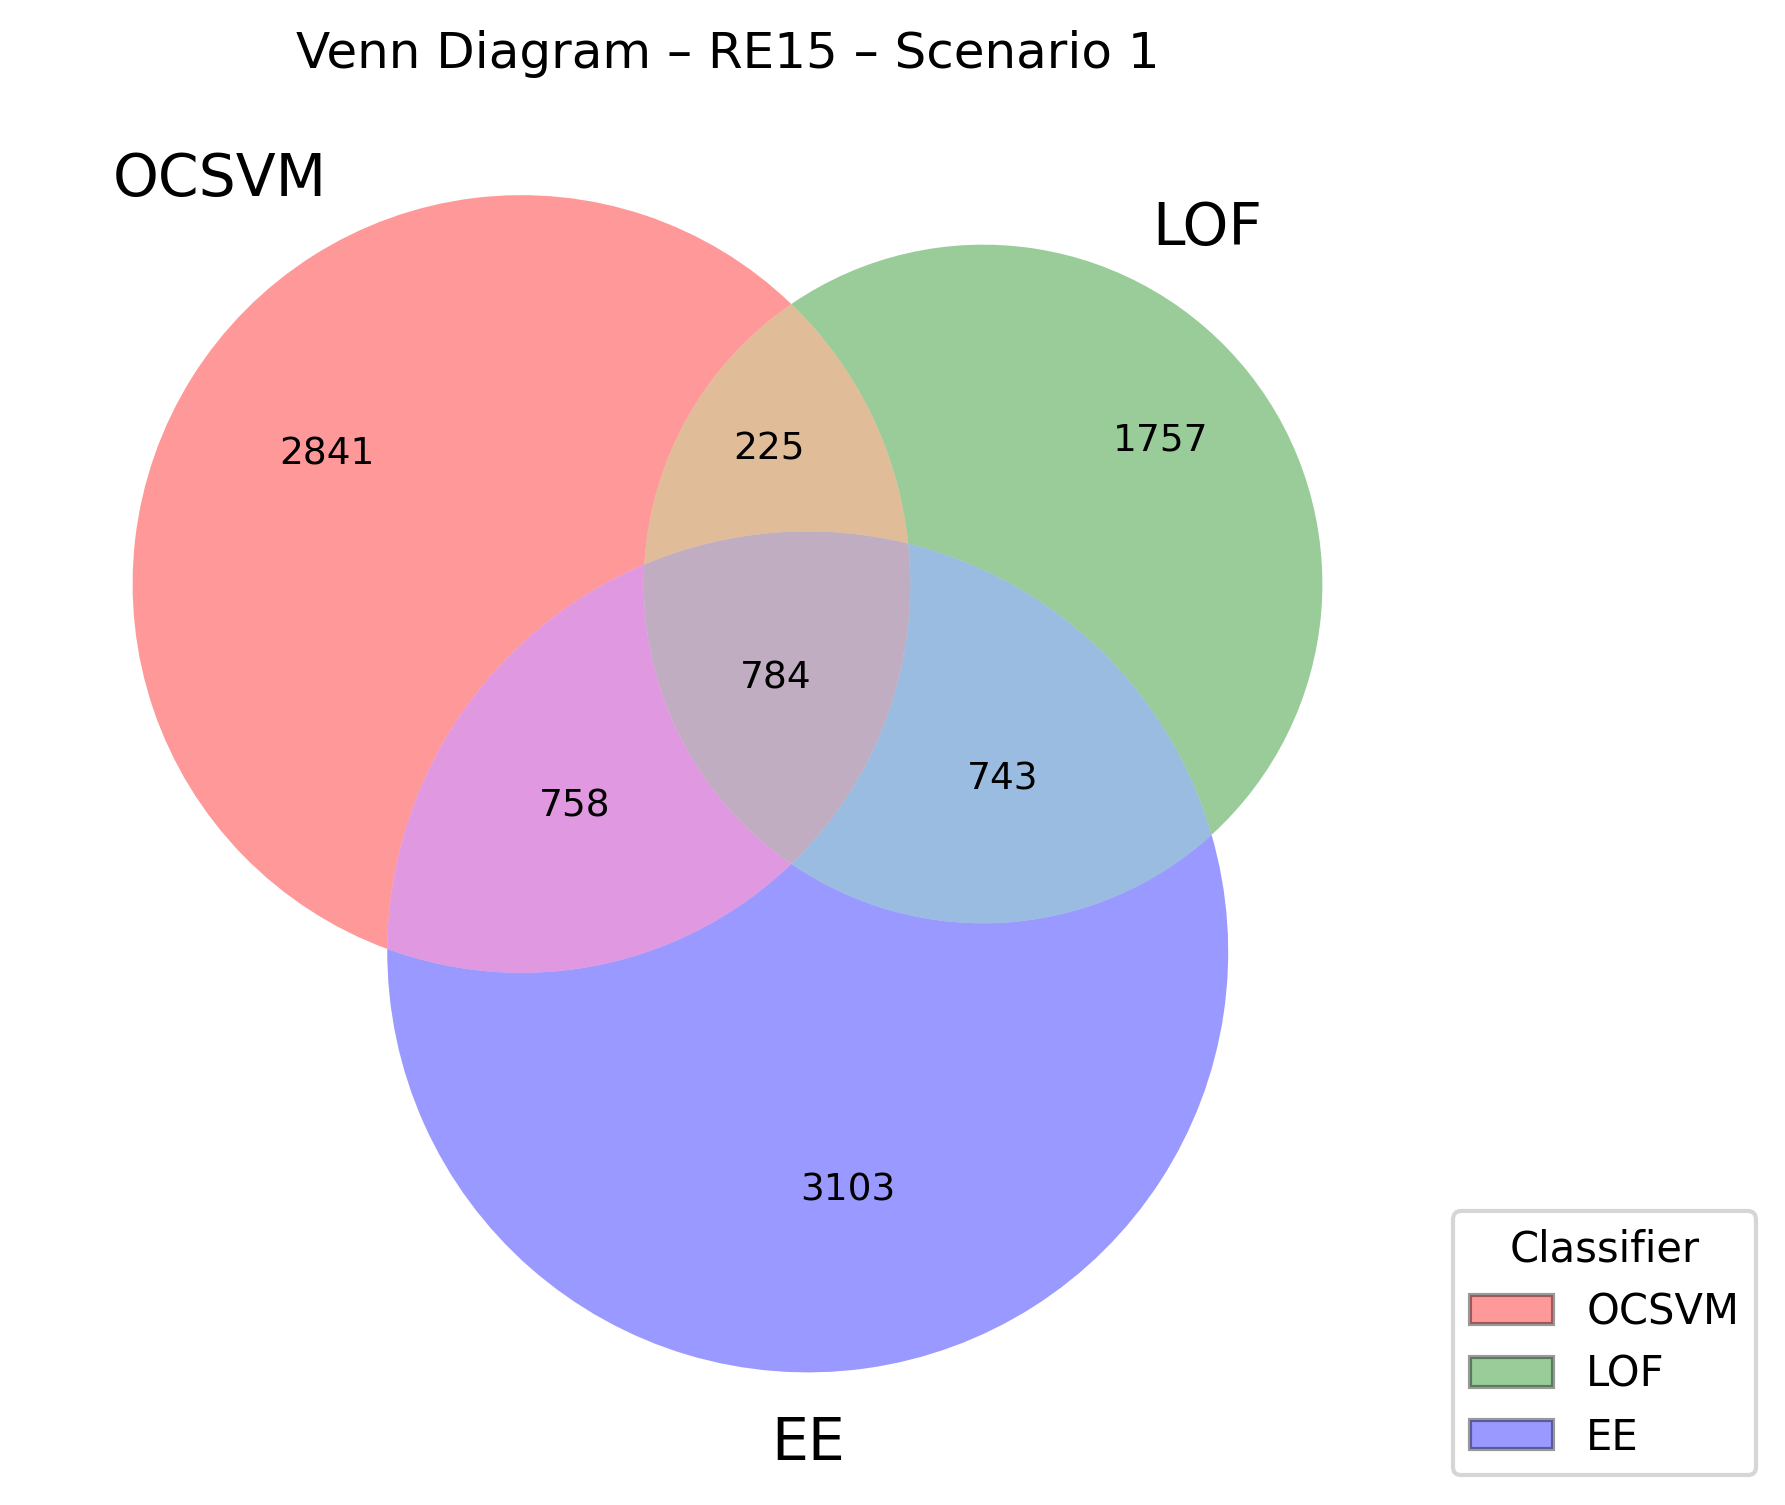
\includegraphics[width=\linewidth]{chapters/venn_re15_s1.png}
        \caption{Scenario 1}
    \end{subfigure}\hfill
    \begin{subfigure}[t]{0.32\linewidth}
        \centering
        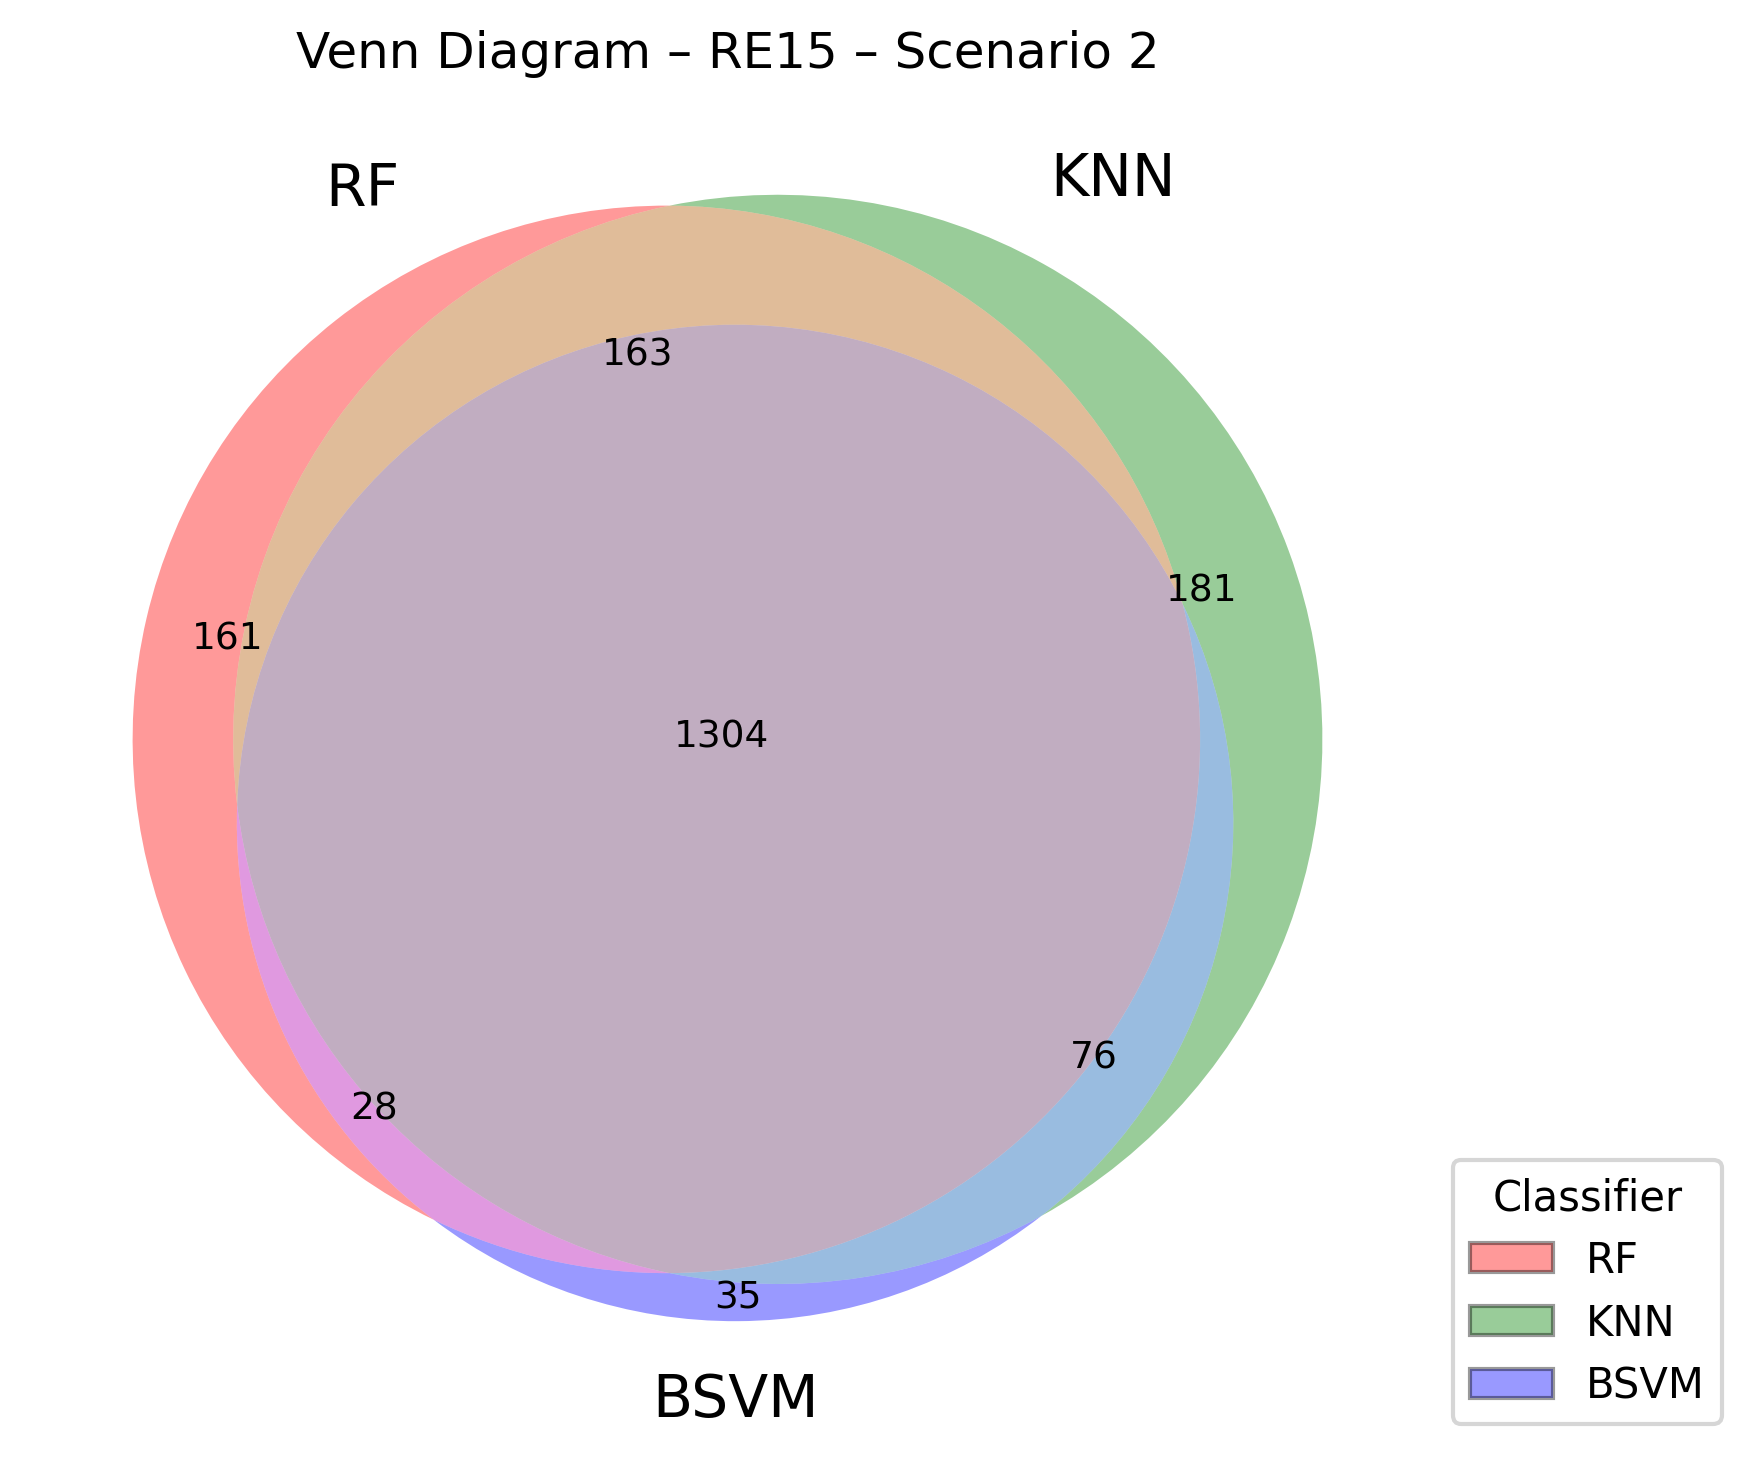
\includegraphics[width=\linewidth]{chapters/venn_re15_s2.png}
        \caption{Scenario 2}
    \end{subfigure}\hfill
    \begin{subfigure}[t]{0.32\linewidth}
        \centering
        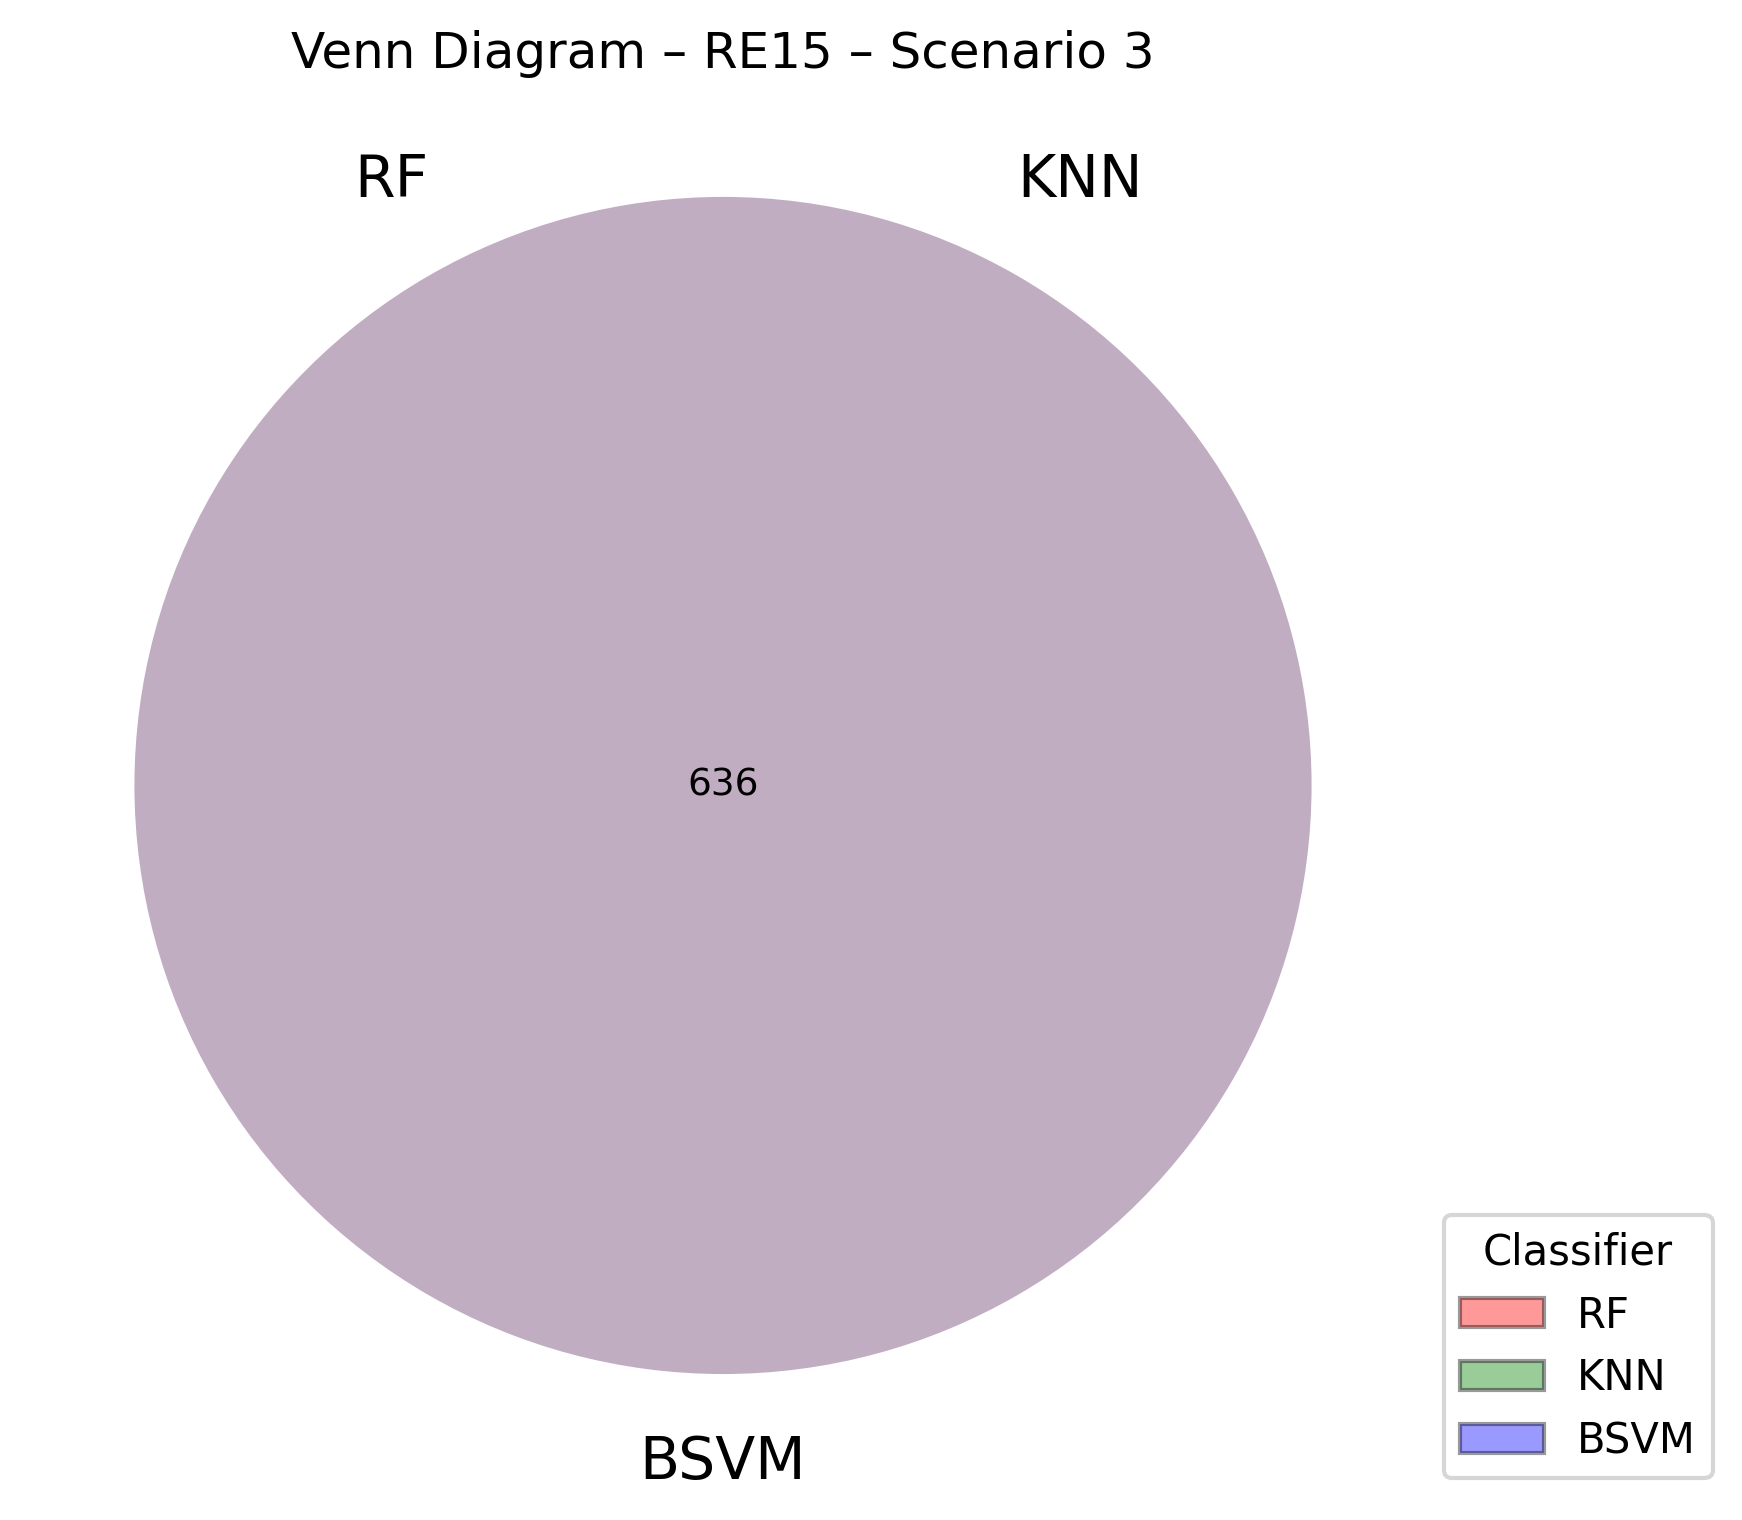
\includegraphics[width=\linewidth]{chapters/venn_re15_s3.png}
        \caption{Scenario 3}
    \end{subfigure}
    \caption{Error overlaps (Venn diagrams) for the RE15 representation.}
    \label{fig:venn-re15}
\end{figure}

\paragraph{RE15 Representation}

For the RE15 representation, the overlap structure changes across
scenarios. In Scenario~1, the diagrams show considerable classifier-
specific error regions (\cref{fig:venn-re15}), meaning that each model misclassifies a
substantial number of samples that the others classify correctly.
Although a triple overlap exists, it is not dominant, indicating
divergent decision behavior.

In Scenario~2, the triple intersection becomes the largest region,
while the unique error regions shrink considerably. This indicates
that most misclassifications are shared among all classifiers,
and only a small fraction depends on the model choice.

In Scenario~3, the triple overlap effectively covers the entire
error set. All three classifiers misclassify the same instances,
representing complete agreement in failure cases. Under this
condition, the ensemble classifier cannot improve performance,
since altering the aggregation strategy does not change the
underlying error set.

%{\color{gray} \paragraph{Relation to Ensemble Performance}
%The overlap analysis clarifies the ensemble results observed earlier.
%When classifier errors strongly overlap (large triple intersections),
%ensemble aggregation offers limited gains, as shared errors cannot
%be corrected. Conversely, scenarios with larger classifier-specific
%regions provide more potential for ensemble improvements, since
%disagreement between models allows majority voting or random
%selection to mitigate individual weaknesses.}

\clearpage
\subsection{Runtime and Memory Consumption}
\subsubsection{Runtime}
\begin{figure}[!htbp]
	\centering
	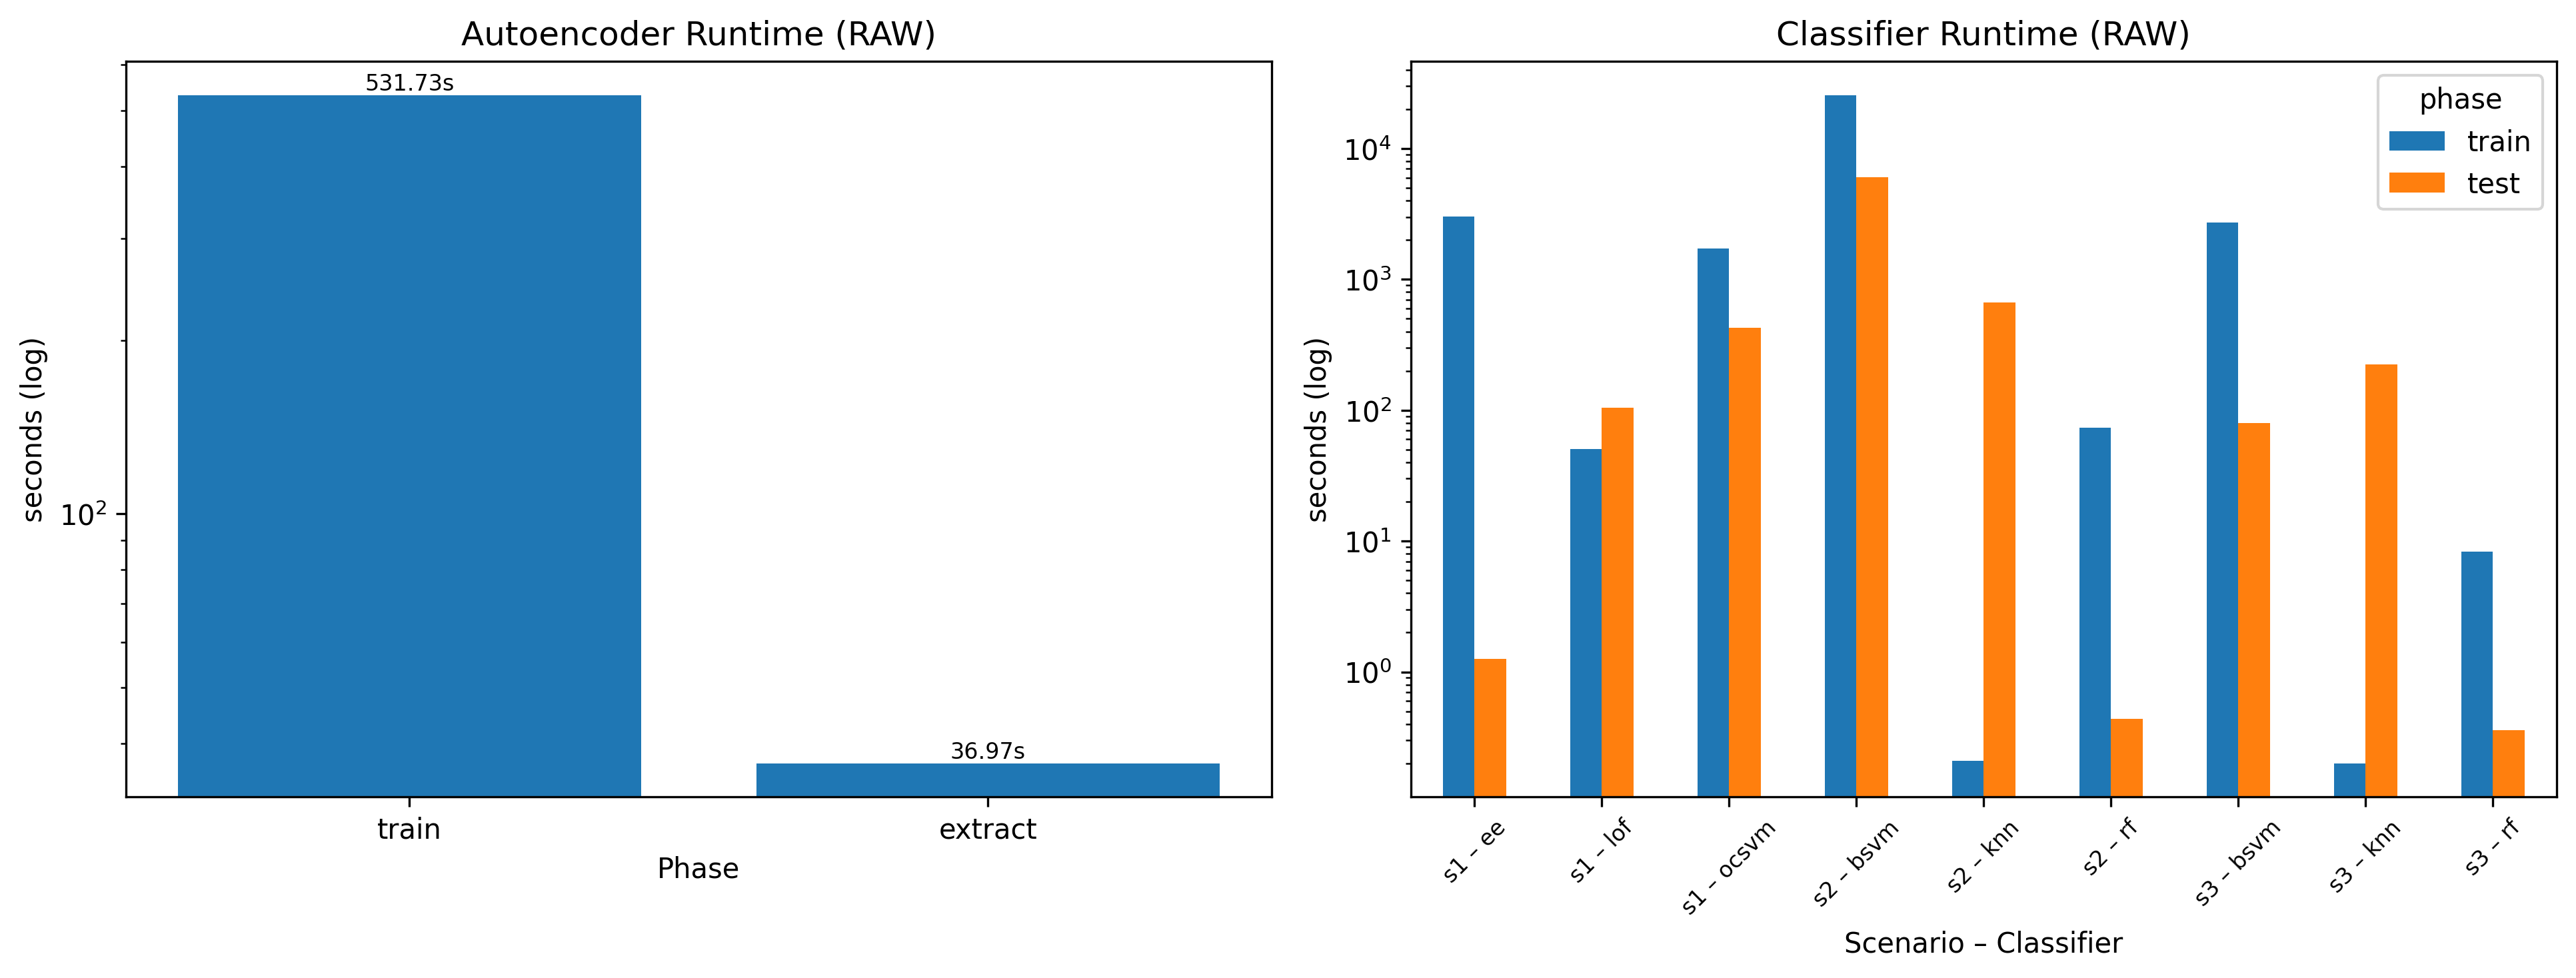
\includegraphics[width=\linewidth]{chapters/runtime_raw.png}
	\caption{Runtime of Feature Extraction and Traditional \ac{ML} Models — RAW}
	\label{fig:runtime-raw}
\end{figure}

For the RAW representation (\cref{fig:runtime-raw}), classifier
runtimes vary drastically across models and scenarios.
In general, training requires more time than testing; however,
important exceptions exist.

Binary \ac{SVM} exhibits the highest computational cost, particularly
in Scenario~2, where both training and testing times are extremely
large. Elliptic Envelope and \ac{OCSVM} also incur substantial training
costs in Scenario~1. In contrast, \ac{KNN} has an almost negligible
training time, as it merely stores the training data. Its prediction
phase, however, is significantly more expensive because each test
instance requires distance computations to many stored samples.
This asymmetry is especially pronounced for RAW features.

Random Forest achieves comparatively small testing times,
particularly in Scenarios~2 and~3, where predictions are performed
in sub-second ranges. Overall, for RAW features the classifier
choice strongly influences total runtime, with \ac{SVM}-based models
and \ac{KNN} representing the main computational bottlenecks.

\begin{figure}[!htbp]
	\centering
	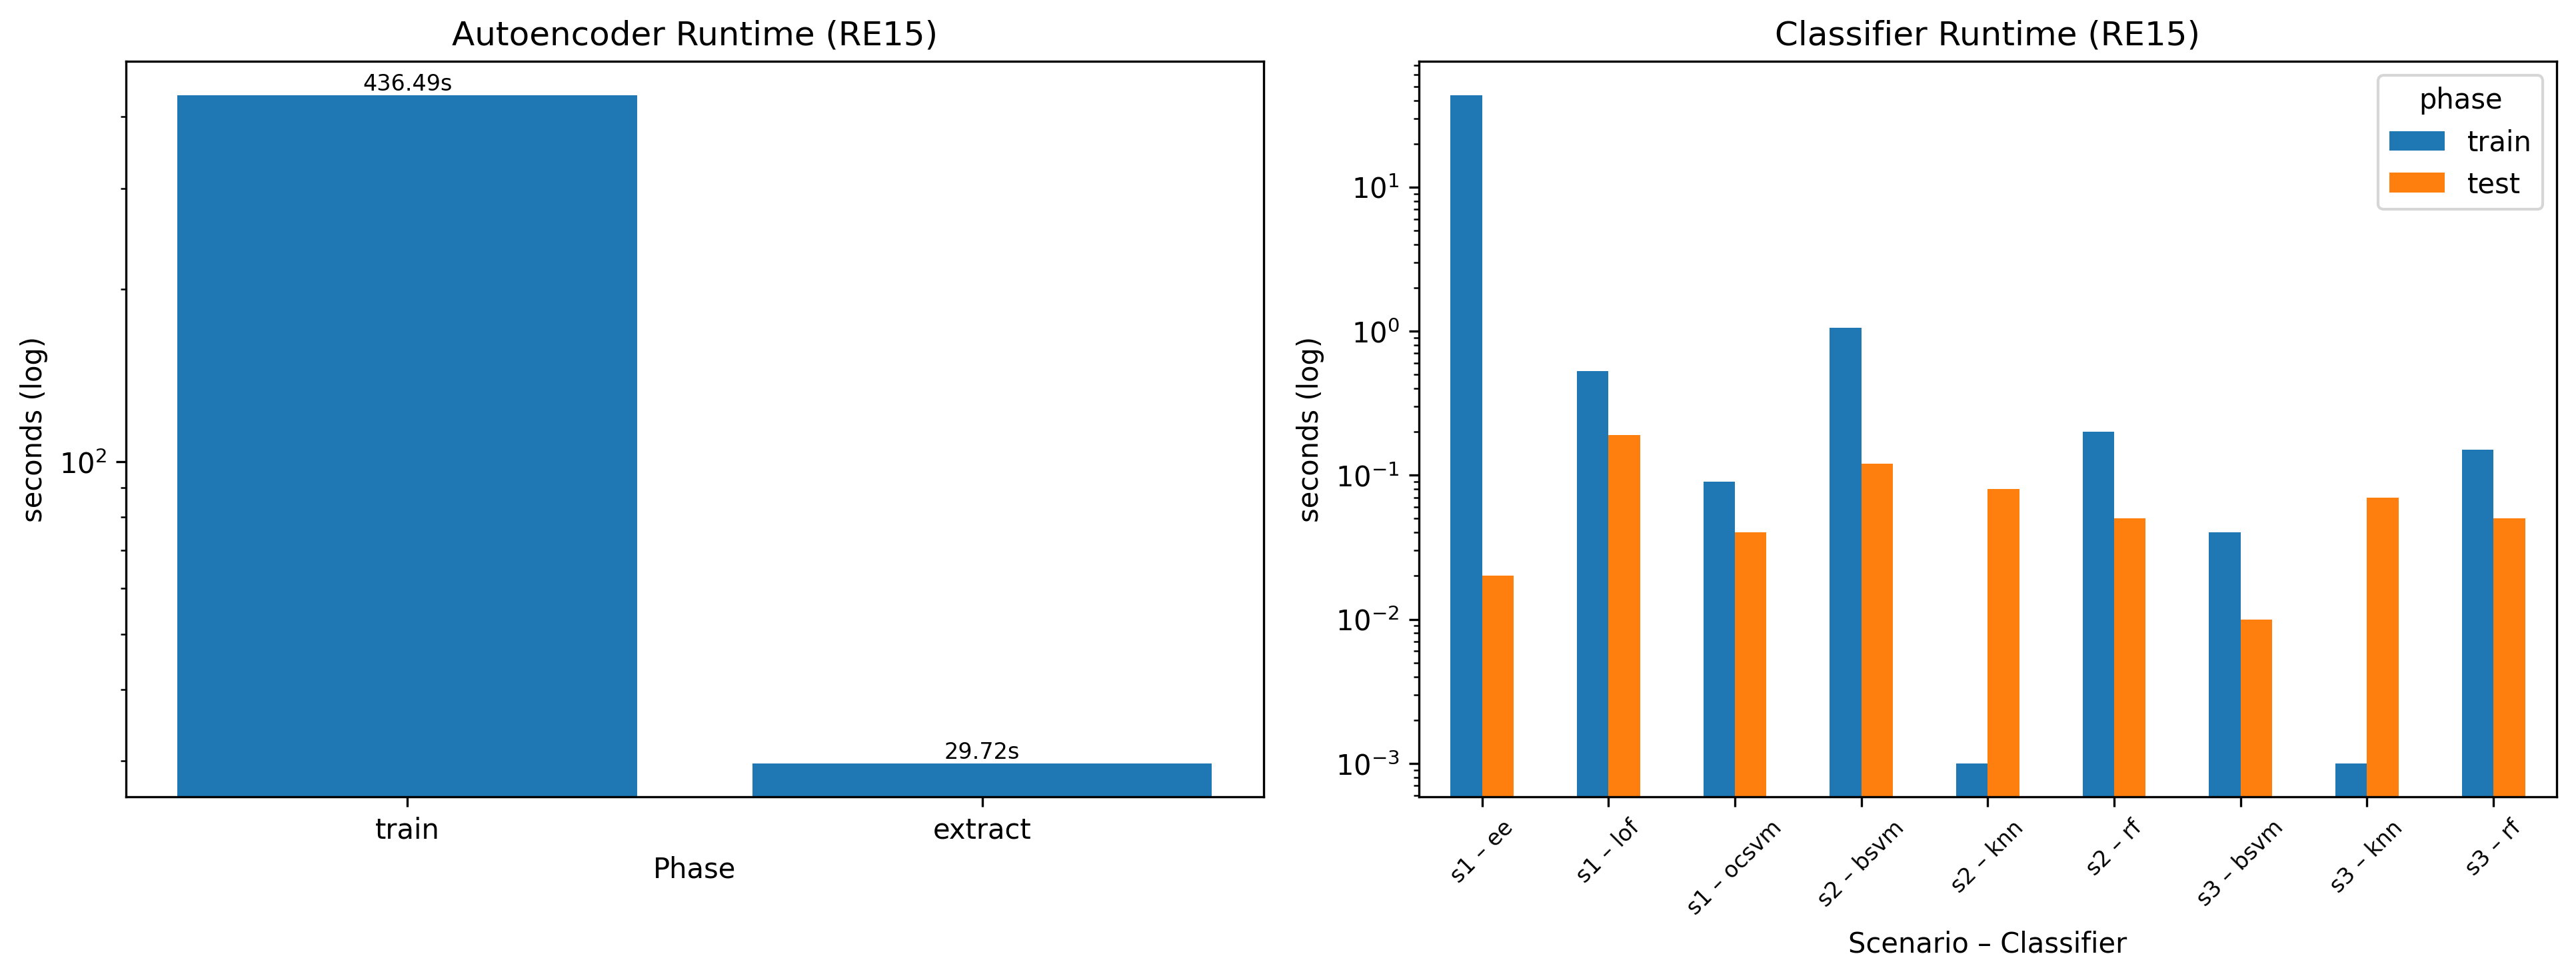
\includegraphics[width=\linewidth]{chapters/runtime_re15.png}
	\caption{Runtime of Feature Extraction and Traditional ML Models — RE15}
	\label{fig:runtime-re15}
\end{figure}

When using the RE15 representation (\cref{fig:runtime-re15}),
classifier runtimes decrease dramatically.
Except for Elliptic Envelope, whose training time remains
noticeably higher than the others, most classifiers operate
within sub-second to approximately one-second ranges during
training. Testing times are consistently small and relatively
similar across models.

In this setting, the classifier stage is no longer the dominant
cost factor. Instead, the primary computational overhead stems
from the feature extraction step (autoencoder training),
while the subsequent classification becomes comparatively
lightweight.

Overall, the results indicate that RAW representations impose
significant computational demands at the classifier level,
whereas RE15 substantially reduces classifier runtime,
shifting the computational burden primarily to feature
extraction.

\subsubsection{Memory Consumption}

\begin{figure}[!htbp]
	\centering
	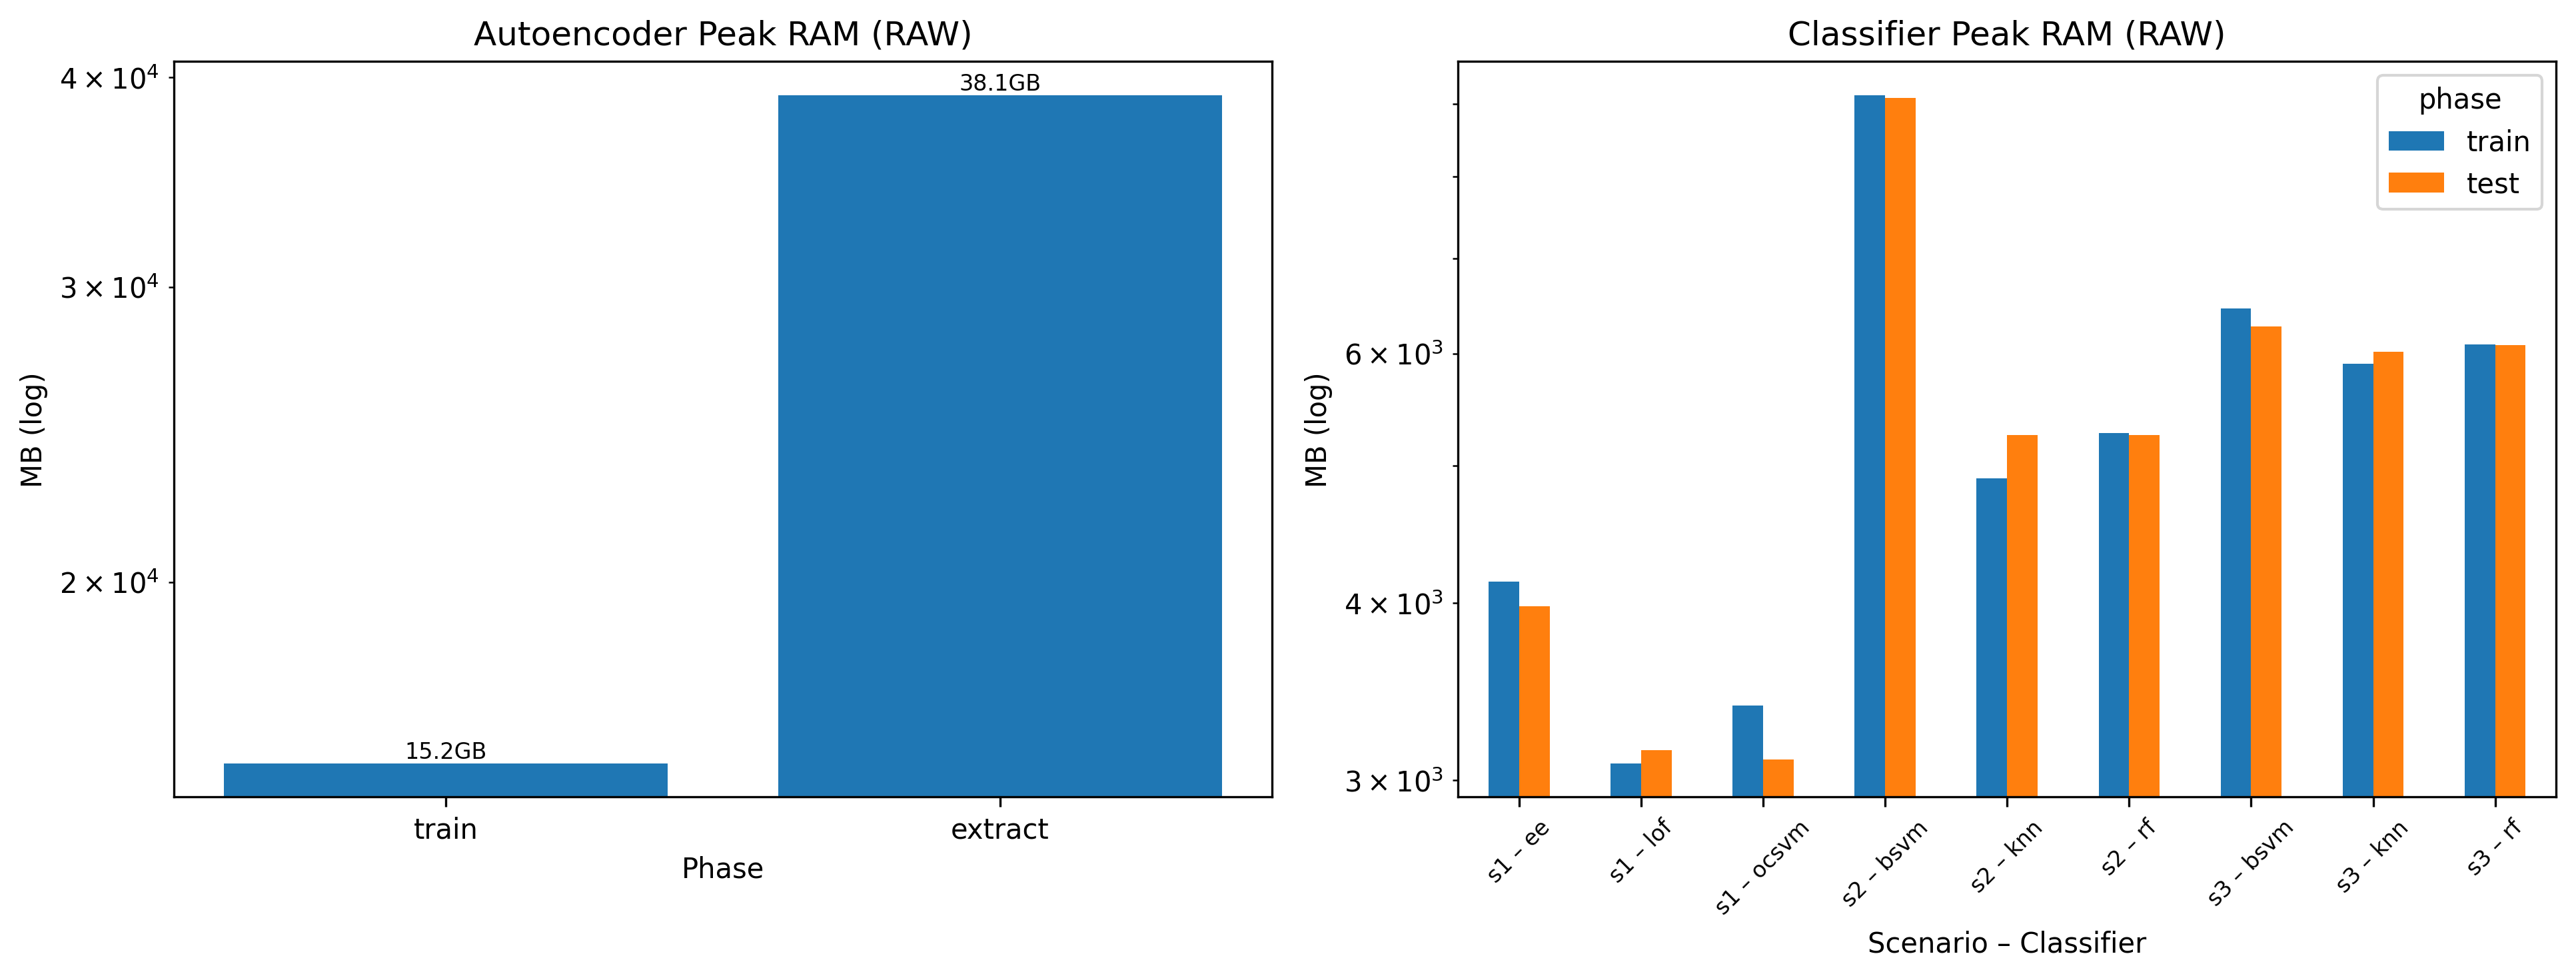
\includegraphics[width=\linewidth]{chapters/ram_raw.png}
	\caption{Memory Consumption — Feature Extraction and Traditional ML Models (RAW)}
	\label{fig:ram-raw}
\end{figure}

For the RAW representation (\cref{fig:ram-raw}), the feature extraction
stage dominates overall memory usage. While autoencoder training already
requires substantial memory, the encoding (feature extraction) phase
reaches the highest peak RAM values within the entire pipeline.
This indicates that processing and storing large byte-vector batches
constitutes the primary memory bottleneck.

In contrast, classifier memory usage remains moderate relative to
feature extraction. For RAW features, peak RAM consumption varies
considerably across scenarios. Scenario~1 exhibits comparatively low
memory usage, whereas Scenarios~2 and~3 require significantly more
memory. The highest peak occurs for Binary \ac{SVM} in Scenario~2,
reflecting the cost of handling high-dimensional feature spaces
with large training sets.

Across classifiers, training and testing phases show similar
memory profiles, indicating that model size and stored data
structures dominate memory requirements rather than temporary
computation during prediction.



\begin{figure}[!htbp]
	\centering
	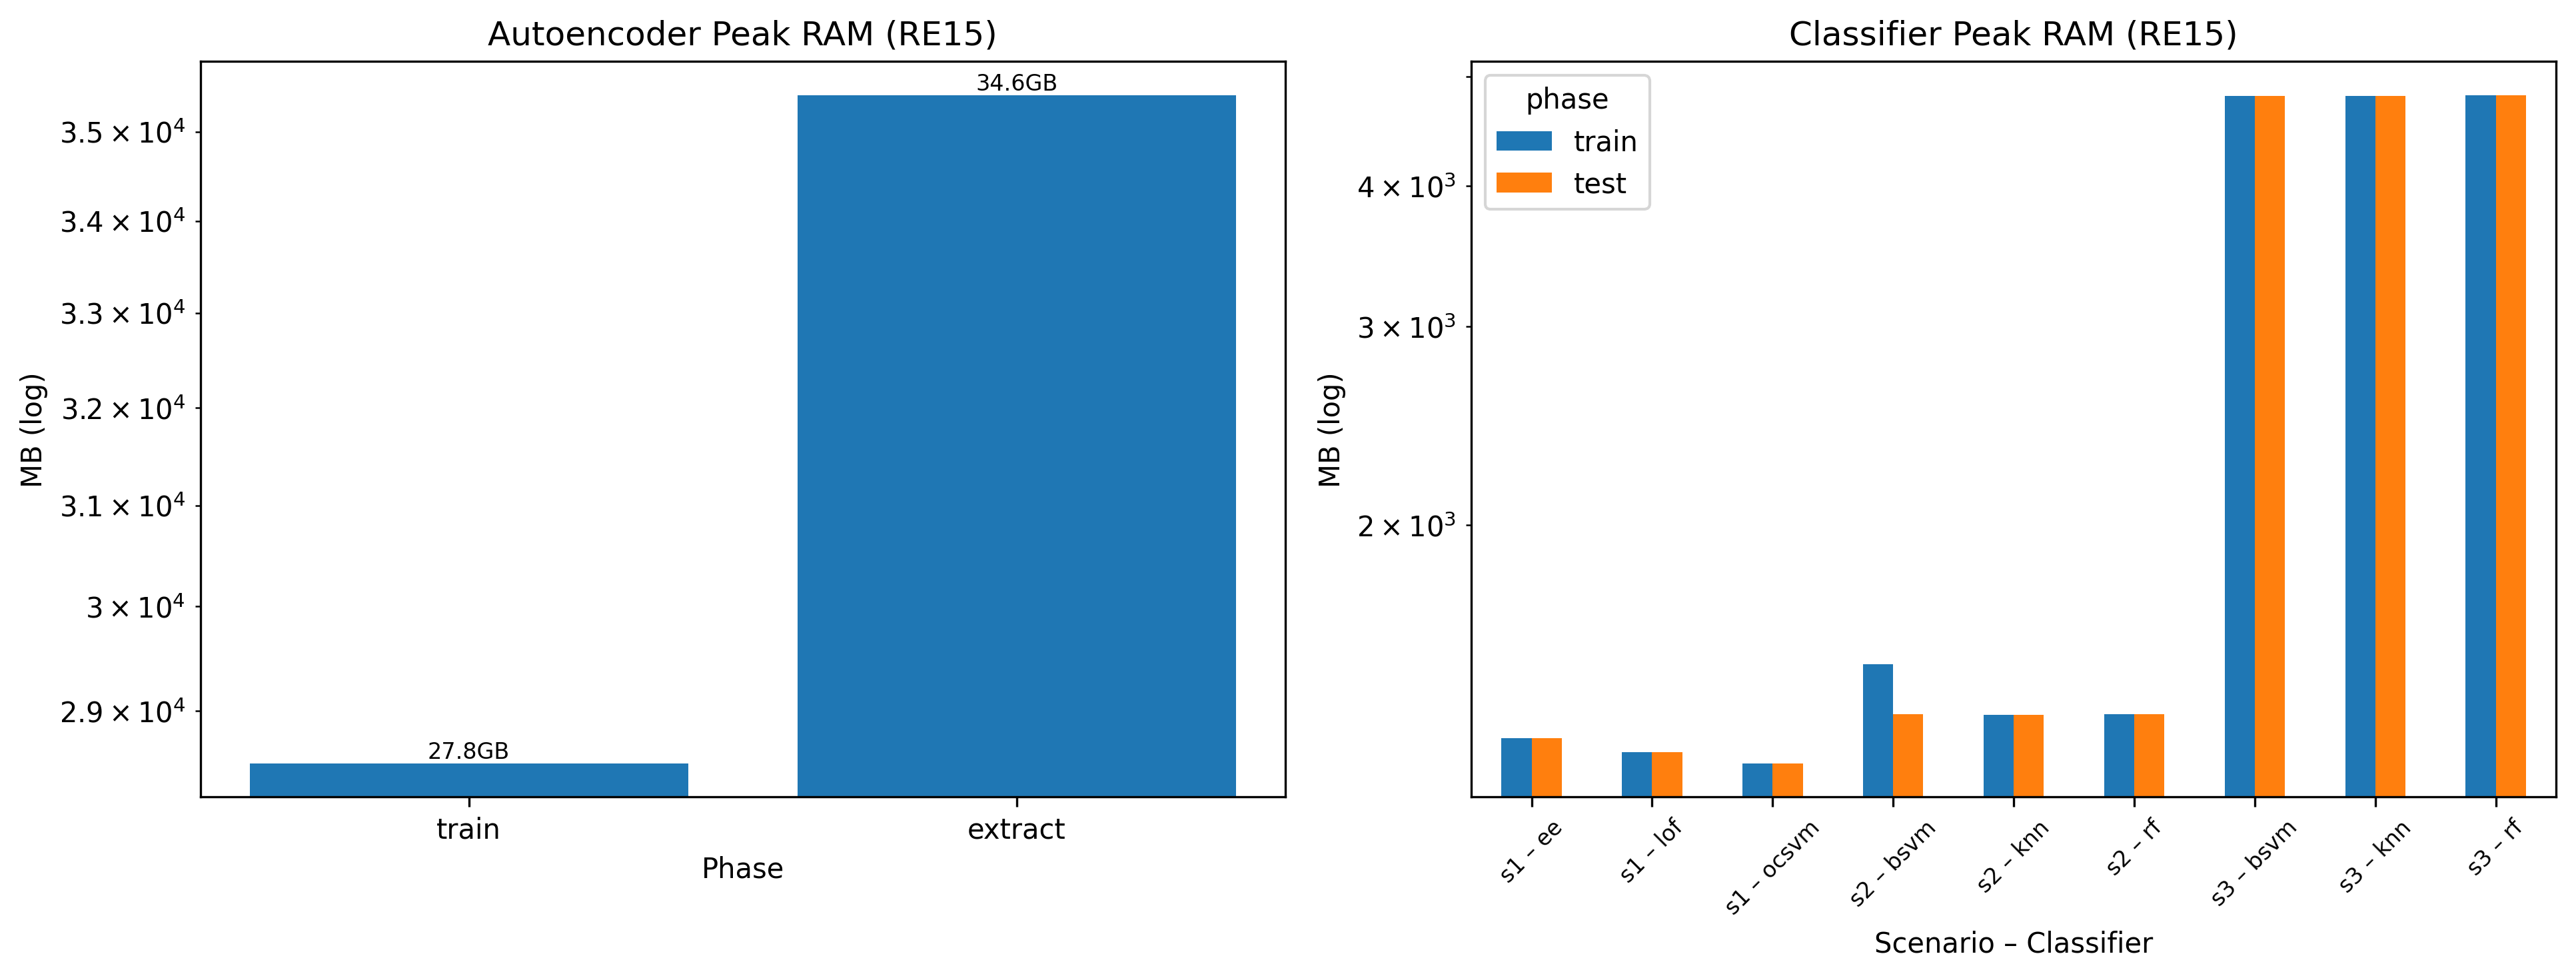
\includegraphics[width=\linewidth]{chapters/ram_re15.png}
	\caption{Memory Consumption — Feature Extraction and Traditional ML Models (RE15)}
	\label{fig:ram-re15}
\end{figure}

For the RE15 representation (\cref{fig:ram-re15}), overall memory
consumption is reduced compared to RAW, particularly at the
classifier stage. Nevertheless, the autoencoder remains the most
memory-intensive component. Interestingly, autoencoder training
requires more memory for RE15 than for RAW, suggesting that the
representation structure influences internal activation storage.

Classifier memory usage under RE15 is substantially lower in
Scenarios~1 and~2, but increases noticeably in Scenario~3.
This scenario-dependent behavior indicates that dataset composition
(e.g., class distribution and sample count) has a strong influence
on memory allocation.

Overall, RAW exhibits lower memory in Scenario~1 but significantly
higher memory in Scenarios~2 and~3, whereas RE15 maintains low
memory usage in the first two scenarios but shows a marked increase
in Scenario~3.


\section{\ac{DL} Models}

\begin{figure}[htb]
	\centering
	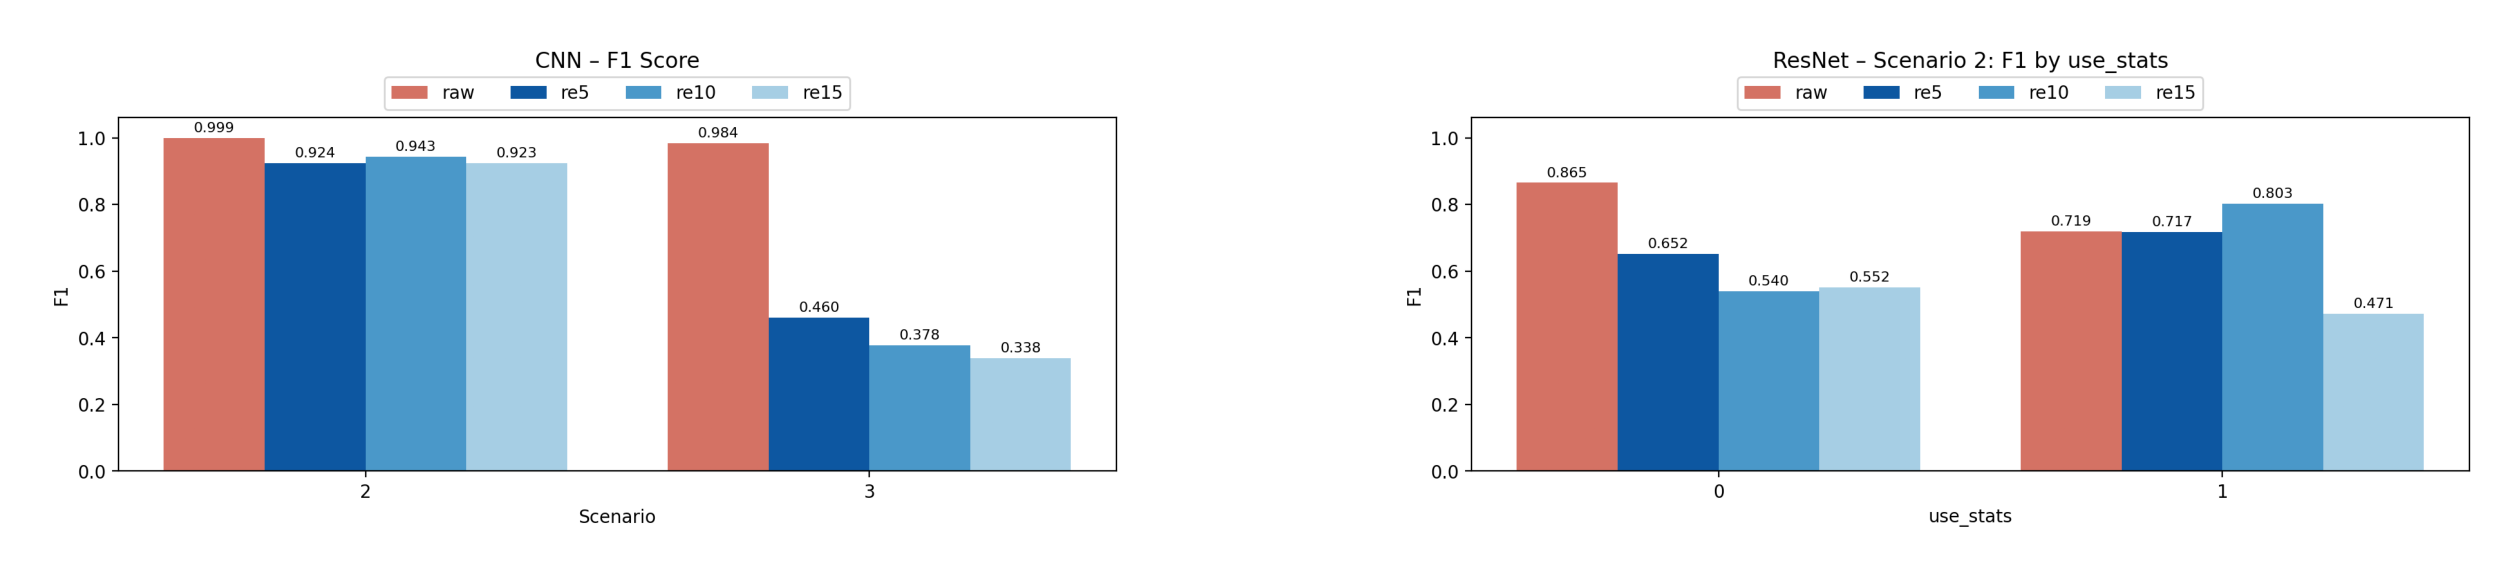
\includegraphics[width=\linewidth]{chapters/cnn_and_resnet_side_by_side.png}
	\caption{F1-scores of the CNN and ResNet classifiers across dataset representations}
	\label{fig:cnn-resnet}
\end{figure}

\subsection{\ac{CNN} Results}

The left panel of \cref{fig:cnn-resnet} summarizes the F1-scores of the
\ac{CNN} classifier for Scenarios~2 and~3 across the four dataset
representations (RAW, RE5, RE10, RE15). All \ac{CNN} models were trained
with oversampling to mitigate class imbalance effects.

Across all dataset types, Scenario~2 achieves consistently strong
performance. F1-scores exceed 0.9 for every representation,
with near-perfect detection for the RAW dataset. This indicates
that when sufficient labeled data and attack diversity are available,
the CNN can effectively learn discriminative byte-level patterns.

Although the reverse-engineered representations perform slightly
worse than RAW in Scenario~2, the differences among RE5, RE10,
and RE15 remain relatively small. Among them, RE10 achieves the
highest F1-score, suggesting that this representation offers a
balanced trade-off between compression and preserved structure.
Overall, the \ac{CNN} appears capable of partially compensating for
information loss in reduced representations when attack diversity
is sufficient.

In contrast, Scenario~3 shows a substantial performance drop for
all reverse-engineered datasets. Despite oversampling, F1-scores
decrease markedly, indicating limited generalization capability.
A likely explanation is the restricted diversity of attack types
in this scenario. While oversampling increases the number of
training instances, it does not introduce additional structural
variation, which limits the model’s ability to learn robust
decision boundaries.

Notably, the RAW representation maintains strong performance even
in Scenario~3. This suggests that full packet information provides
rich structural cues that remain discriminative even under
constrained attack configurations. In comparison, the
reverse-engineered representations appear to be limited more by
representational expressiveness than by class imbalance alone.

\subsection{ResNet}
The results obtained with the ResNet classifier in Scenario 2 show a clear impact of both reverse engineering and the inclusion of statistical features. When using raw packets without reverse engineering, the model achieved an F1-score of 0.865 without statistical features and 0.719 when statistical features were included. This indicates that raw packet information alone already provides strong discriminative signals for the classifier.

After applying reverse engineering, where only sequences of physical readings were used, the performance decreased. For p = 5, the F1-score dropped to 0.652, and further decreased to 0.540 for p = 10. A slight improvement was observed for p = 15, reaching 0.552, but the performance remained significantly below the raw packet baseline.

When statistical features were added to the ResNet input, their impact depended on the sequence length. For p = 5, the performance slightly improved to 0.717, suggesting that the additional statistical context helped compensate for the loss of structural packet information. For p = 10, the F1-score further increased to 0.803, representing the best result among the reverse-engineered inputs. However, for p = 15, the performance dropped significantly to 0.471, indicating that larger physical-reading sequences combined with statistical features may introduce noise or redundant information that negatively affects classification performance.

Overall, these results show that ResNet can effectively learn patterns from raw packet bytes, while its performance becomes more sensitive when only partial packet information is available.



\textbf{Comparison CNN ResNet}
A comparison between CNN and ResNet shows noticeable differences in their robustness across scenarios. For raw packets, both models achieved high performance, with CNN slightly outperforming ResNet, reaching an F1-score close to 0.999, while ResNet achieved 0.865. This indicates that CNN is particularly effective at learning local byte-level patterns in raw packet structures.

However, when reverse engineering was applied and only partial packet data was used, both models experienced a decline in performance. The CNN showed a sharper drop in Scenario 3, whereas the ResNet demonstrated more stable behavior when statistical features were included. In particular, ResNet benefited from the additional statistical features in some configurations, reaching 0.803 for p = 10, which suggests that the deeper architecture and residual connections may help integrate heterogeneous input features more effectively.

In summary, CNN achieves the best performance when complete packet structures are available, while ResNet shows slightly better adaptability when additional statistical features are incorporated into the model.

\section{Other Anomaly Detection Methods}
\begin{figure}[!htbp]
	\centering
	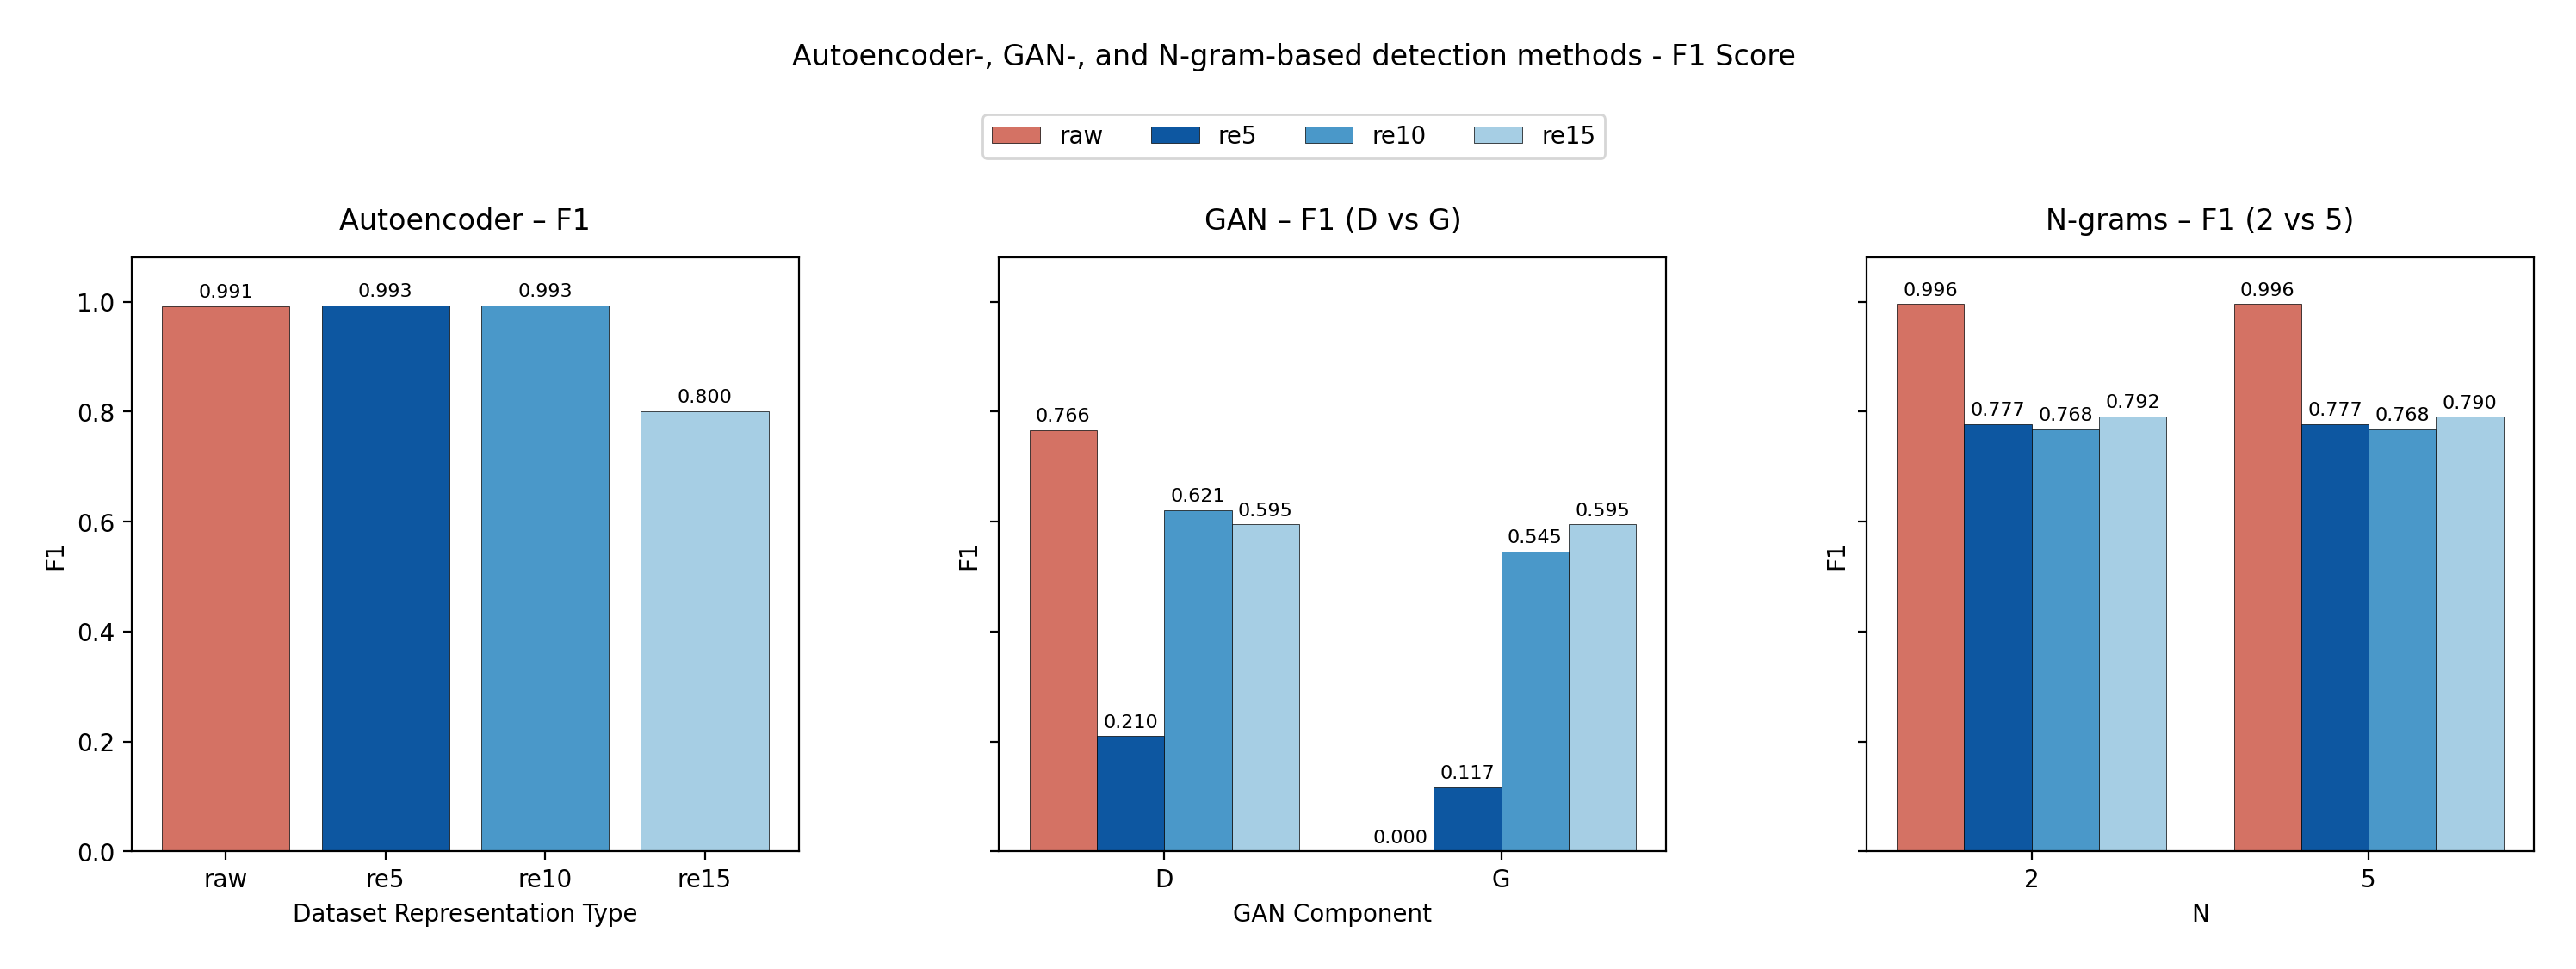
\includegraphics[width=\linewidth]{chapters/ae_gan_ngram_f1_combined.png}
	\caption{Autoencoder, GAN and N-Gram -based detection F1-Score}
     \label{fig:ae-gan-ngram}
\end{figure}


\textbf{Autoencoder}

The left panel of \cref{fig:ae-gan-ngram} summarizes the F1-scores of
the reconstruction-error-based \ac{SDA} classifier across the
different dataset representations (RAW, RE5, RE10, RE15).

For RAW, RE5, and RE10, the autoencoder achieves near-perfect
classification performance, with F1-scores close to 1.0.
Both precision and recall remain consistently high in these settings,
indicating that the learned reconstruction threshold effectively
separates benign and malicious traffic. Compared to RAW, the RE5
and RE10 representations even show slightly higher precision and
F1-scores, suggesting that moderate reverse engineering does not
degrade the discriminative power of the reconstruction-based method.

In contrast, performance drops dramatically for RE15.
The F1-score decreases sharply, accompanied by both low recall
and low precision. The reduced recall indicates that many attack
instances are incorrectly classified as benign (false negatives),
while the low precision reflects a substantial proportion of
false positives among predicted attacks. This behavior suggests
that the RE15 representation no longer preserves sufficient
structure for reliable reconstruction-based anomaly detection.

Overall, the results demonstrate that the \ac{SDA}-based
approach is highly effective for RAW and moderately reduced
representations (RE5, RE10), but becomes unstable when the
reverse-engineered representation is further compressed.

\textbf{GAN}

As shown in the middle panel of figure~\ref{fig:ae-gan-ngram}, the performance of the GAN-based approach is highly unstable and significantly lower compared to the other evaluated methods. While the discriminator achieves better results than the generator-based detection, its performance remains inferior to that of the \ac{SDA} and the N-gram models.

In particular, generator-based anomaly detection struggles considerably, especially when applied to raw packet data. We attribute this behavior to the inherent difficulty of generating valid raw network packets from random noise. Raw packets follow strict structural and syntactic constraints, including precise byte-level patterns and protocol-specific rules. Even minor deviations from these constraints can result in unrealistic or invalid packet representations.

Due to this high structural rigidity, the generator faces substantial challenges in learning an accurate representation of the underlying packet distribution. Consequently, the generated samples often fail to approximate realistic packet structures, leading to weaker anomaly detection performance.


\textbf{N-Gram}


The N-gram-based detection method demonstrates outstanding performance when applied to raw packet data, achieving an F1-score of approximately 0.996 as shown in the right panel of figure \ref{fig:ae-gan-ngram}. This near-perfect performance indicates that raw network packets contain highly distinctive local byte-sequence patterns that can be effectively captured by N-gram representations. Since raw packets include both protocol headers and payload information, they preserve structural regularities and fixed byte-level dependencies that strongly differentiate normal and malicious traffic.

After applying reverse engineering and restricting the input to physical readings only, a noticeable decrease in performance can be observed. Although the F1-score drops compared to the raw packet scenario, it remains relatively stable across different values of the concatenation parameter 
$p$. This stability suggests that increasing the number of concatenated physical readings does not significantly enhance or degrade the discriminating capability of the N-gram model.

The comparison between 2-gram and 5-gram configurations shows only marginal differences in performance. This indicates that extending the N-gram length does not substantially improve detection accuracy. In practice, shorter byte dependencies already capture most of the relevant structural information present in the packets. Larger N-grams may increase representational complexity, but they do not provide a significant additional benefit in this context.

The overall performance reduction observed after reverse engineering can be explained by the removal of protocol-related bytes. Raw packets contain strict and repetitive structural patterns defined by the underlying communication protocol. These regular patterns are highly suitable for modeling with N-grams, as they rely on local sequential dependencies. In contrast, physical readings are more variable and less structured at the byte level. As a result, the statistical regularities that N-grams exploit become weaker, leading to a reduced but still stable detection performance.


\textbf{Comparison AE, GAN, N-Gram}

Overall, the experimental results indicate that \ac{SDA}-based approaches provide the most robust and consistent performance across all evaluated scenarios. In particular, the stacked denoising autoencoder (SDA) maintains stable detection accuracy not only on raw packet data but also after reverse engineering and data reduction. This robustness suggests that representation-learning methods are well-suited for modeling both protocol-level structures and higher-level behavioral patterns in ICS traffic, even when structural information is partially removed.

The N-gram-based approach also demonstrates strong performance, especially when applied to raw packet data. Its effectiveness can be attributed to its ability to capture local byte-level patterns and repetitive protocol structures. However, its performance degrades once the input is restricted to physical readings only, indicating that it relies heavily on the structural regularities present in complete packet data. While N-grams remain competitive, their dependence on raw packet structure limits their generalizability in scenarios where protocol information is unavailable or intentionally removed.

In contrast, GAN-based methods exhibit unstable and comparatively weak performance. Although the discriminator performs moderately better than the generator-based detection, the overall results suggest that GANs are not well-suited for reliable anomaly detection at the byte level in ICS environments. The strict structural constraints and deterministic nature of raw network packets make it difficult for the generator to learn a realistic data distribution from noise. Consequently, the generated samples often fail to approximate valid packet structures, which negatively impacts detection performance.

In summary, representation-learning approaches such as autoencoders appear to be the most reliable choice for anomaly detection in proprietary ICS traffic. N-grams offer strong performance when full structural information is available, whereas GAN-based models struggle to provide stable and trustworthy results in this highly structured and safety-critical domain.

\section{Summary}


This section summarizes the main observations across all evaluated
approaches.

\subsection{Overall Model Performance}

Across all experiments, the strongest overall performance is achieved
by the reconstruction-based \ac{SDA}, the N-gram model,
and the \ac{CNN} classifier in Scenario~2.
In this setting, F1-scores approach near-perfect classification,
particularly for the RAW representation.

In contrast, GAN-based detection and traditional machine learning
classifiers exhibit the weakest overall performance.
While GAN models show moderate success in some configurations,
their results remain substantially below those of autoencoder- and
CNN-based approaches.
Traditional \ac{ML} classifiers are especially sensitive to the chosen
representation and scenario and frequently suffer from significant
performance degradation.

\subsection{Influence of Dataset Representation}

The RAW packet representation consistently yields the best results
across nearly all model families.
It preserves the full structural and contextual information of
network traffic, enabling both deep learning and classical models
to extract highly discriminative patterns.

The reverse-engineered representations (RE5, RE10, RE15) introduce
progressive aggregation and information reduction.
Among them, RE15—representing the strongest compression—produces
the weakest overall performance.
This indicates that aggressive abstraction of packet structure
removes discriminative signals that are essential for reliable
attack detection.

\subsection{Impact of Reverse Engineering Across Model Families}

The influence of reverse engineering differs substantially
between model classes.

Deep learning architectures such as \ac{CNN}, \ac{SDA},
and ResNet show comparatively robust behavior.
Although minor performance reductions occur for reduced
representations, these models remain competitive,
particularly when sufficient labeled data is available.
This suggests that deep architectures can internally learn
hierarchical feature representations that partially compensate
for information loss.

GAN-based and N-gram models exhibit moderate performance
degradation under reverse-engineered representations.
While still functional, their discriminative capacity decreases
more noticeably than for \ac{CNN} or \ac{SDA}.

The strongest negative impact is observed for traditional
machine learning classifiers.
These approaches rely explicitly on the extracted latent feature
vectors and do not perform hierarchical representation learning.
Consequently, they are more sensitive to the loss of structural
information introduced by reverse engineering.

\subsection{Impact of Evaluation Scenario}

Scenario characteristics have a strong influence on performance
across all models.
Scenario~2 consistently achieves the highest F1-scores,
indicating that models perform best when attack types are well
represented during training.

Scenario~3 yields the lowest overall performance.
The presence of unseen or highly constrained attack types
significantly reduces generalization capability, even for
strong deep learning models.
This highlights that attack diversity during training plays a
more decisive role than class imbalance alone.


